%\documentclass[oneside,final,14pt]{article}
\documentclass[a4paper, 12pt, onecolumn]{extarticle}
%\documentclass[a4paper, 9pt, twocolumn]{extarticle}
\usepackage[utf8]{inputenc}
\usepackage[english]{babel}
\usepackage{vmargin}
\usepackage{amsmath}
\usepackage{amsthm}
\usepackage{graphicx}
%\linespread{1.5}
%\setpapersize{A4}
\setmarginsrb{1.5cm}{2cm}{1.5cm}{1cm}{0pt}{0mm}{0pt}{0mm}
\usepackage{indentfirst}
\usepackage{titlesec}
\usepackage{cite}
\usepackage[dvipsnames]{xcolor}
%\titleformat{\section}[block]{\normalfont\large\bfseries\centering}{\thesection}{1ex}{}
\usepackage[margin=9pt,labelsep=period,font=small,figurename=Fig.]{caption}
%\usepackage[export]{adjustbox}
\usepackage{enumerate}
\usepackage{multirow}
%\setlength{\mathindent}{0\parindent}
%\setlength{\parindent}{0cm}
\sloppy
\setcounter{secnumdepth}{4}
\begin{document}
%\renewcommand{\thesection}{\arabic{section}.}
%\renewcommand{\thesubsection}{\arabic{section}.\arabic{subsection}}
%\renewcommand{\theparagraph}{}
\newtheorem{theorem}{Theorem}
\author{Vyacheslav A. Trofimov\textsuperscript{1}, Dmitry M. Kharitonov\textsuperscript{2}, Mikhail V. Fedotov\textsuperscript{2}}
\title{Cascading process -- new effective tool for frequency conversion of optical pulse and beam}
\date{\textsuperscript{1} South China University of Technology, Guangzhou 510641, China\\
\textsuperscript{2}Lomonosov Moscow State University, Leninskye Gory, Moscow 119992, Russia}
\maketitle
% \begin{large}
% \centerline{Lomonosov Moscow State University, Leninskye Gory, Moscow 119992, Russia}
% \end{large}
\section*{Abstract}
As it is well-known, a frequency conversion is a very important problem of nonlinear optics. The frequency doubling, and a generation of a wave with sum or difference frequency, and the frequency trebling are widely investigated. As a rule, the third harmonic generation (THG) is realized by using one of the following generation schemes. In the first one, firstly the second harmonic generation (SHG) occurs in a medium with the quadratic nonlinear response and then in the second (or in the same) crystal, a wave with the sum frequency is generated. In the second scheme, a generation of a wave with the trebled frequency achieves in a medium with a cubic nonlinear response.

One more process, which is attracted big attention of the scientific community due passed three decades, is the cascading SHG, which is accompanied by the pulse self-action. Early the self-focusing or defocusing of a laser beam and compression or decompression of the laser pulse, caused by the cascading SHG, have been investigated theoretically and experimentally. However, only self-modulation process arising from an effective (induced) cubic nonlinear response in a medium with the quadratic susceptibility is taken into account. Meanwhile, the induced cubic nonlinear response may result in a frequency tripling process under certain conditions. In this paper, we propose using of the cascading SHG for the frequency tripling as a new tool that can be applied for a generation of high optical harmonics.
\section{Introduction}
The cascaded \(\chi^{(2)}\) nonlinear phenomenon remains of interest for many years due to its various practical applications. For the first time, this phenomena has been theoretically predicted in 1974 by A.P. Sukhorukov and Yu.N. Karamzin \cite{bib:n1}. Since 1991 there is a permanent unterest to this phenomenon. So, in 1994, a physical experiment was made by a group of Torruellas \cite{bib:n2}. Then, many researchers have predicted and observed various types of cascading \(\chi^{(2)}\) solitons, in particular, 1D spatial \(\chi^{(2)}\) solitons \cite{bib:n3}, and 2D spatial \(\chi^{(2)}\) solitons \cite{bib:n2, bib:n4, bib:n5}, and \(\chi^{(2)}\) temporal solitons \cite{bib:n6}, and spatio-temporal solitons\cite{bib:n7} and others \cite{bib:n9,bib:n10}. The comprehensive review of observing the cascading \(\chi^{(2)}\) solitons and their practical applications can be found, for example, in \cite{bib:n8}.

One of the cascading SHG applications is the soliton compression \cite{bib:n11, bib:n12, bib:n13, bib:n14, bib:n15, bib:n16, bib:n17, bib:n18}. By choosing the appropriate sign of the phase mismatching, the pulse compression at the fundamental frequency (FF) can be reached. This phenomenon is also of interest nowadays. So, in \cite{bib:n11}, a soliton compression factor about of \(173.52\) is achieved. M. Bache and F.W. Wise have discussed in \cite{bib:n12} the soliton compression at the wavelength \(1030\,nm\) in a LiNbO$_3$ crystal, which length being equal to \(10\,cm\). In \cite{bib:n13} the pulse compression is obtained at the incident pulse with peak power density \(20\,GW/cm^2\). In \cite{bib:n14} such a pulse compression is observed BBO crystal with its length about of \(3\,cm\). 

Big phase mismatching between the wave at the FF and the wave with doubled frequency may lead to self-focusing or defocusing of the beam at the FF, as it was shown in \cite{bib:n19}. In the axial-symmetric case, the beam intensity may be increased about 70 times \cite{bib:n20}. Another important application of the cascading SHG is its using for a laser operating in the so-called free-generation mode, in which a sequence of the pulses with both random durations and random maximal power densities are generated. Therefore, a frequency conversion of these sub-pulses possesses a low efficiency arising from their maximal intensity fluctuations. To suppress these fluctuations, one may use the cascading SHG \cite{bib:n21,bib:n22,bib:n23a,bib:n23} at very low losses of the laser pulse energy: only about \(2\%-3\%\) of the incident energy.

As we see, all the authors, mentioned above, have taken into account the phase self-modulation only for the laser pulse at the FF caused by the cascading SHG. Nevertheless, induced cubic nonlinearity may also lead to THG if the following phase matching conditions occur. Let us suppose that the incident fundamental wave intensity is high enough for manifesting the quadratic nonlinear response of a medium but not remarkable for manifesting of effects corresponding to the third-order susceptibility. We choose a big phase mismatching between waves at the doubled frequency and FF. Therefore, the SH intensity remains low. However, THG (\(\omega_3=3\omega\)) may be observed due to an effective cubic nonlinear response of a medium induced by the cascading SHG if the phase matching between fundamental wave (FW) and a wave at trebled frequency occurs. To analyse and understand the properties of THG under such conditions we derive the equations, describing the frequency tripling process, using the multiscale method (see, for example, \cite{bib:n24}) similar to that presented in \cite{bib:n19}. The modified (new) equations clearly show an appearance of the induced cubic nonlinear response that make possible a high-effective THG. Then, these theoretical results are confirmed by computer simulation results, using a full set of Schr\"{o}dinger equations describing three wave interaction with the frequencies \(\omega,\,2\omega,\,3\omega\). They show that the modified equations approximate the original ones with high precision, and, what is most important, that at least $50\%$ of the incident energy transfers to the third harmonic (TH) wave.

As is well-known, there are different ways to obtain a high efficient THG. The most common way is to use a scheme with two nonlinear crystals. The first crystal is used for the phase-matched SHG, and the second one is used for a phase-matched sum frequency wave generation (SFG) \cite{bib:t4}, \textcolor{ForestGreen}{where $80\%$ efficiency of frequency tripling is achieved experimentally, and up to $100\%$ under theoretical approximation}. There are also several techniques, which lead to reaching of high-efficient THG in a single crystal. For instance, one can use the mirror to change the SH polarisation and realise THG through SFG \cite{bib:t3}. THG in a single BBO crystal with combined quadratic and cubic nonlinear response is realized \cite{bib:t1}. Another technique of the generation is based on the Quasi-Periodic Optical Superlattice (QPOS) \cite{bib:t2}. However, all mentioned methods are not high-effective: the maximum frequency conversion is about \textcolor{blue}{$30\%$} \textcolor{ForestGreen}{$40\%$}.

The advantages of approach, proposed below, are the following. Firstly, only a single nonlinear crystal is required for effective frequency tripling, \textcolor{ForestGreen}{so, our scheme is simpler than the schemes, described above, but still gives promising results}. Secondly, since we require the phase matching for THG and big phase mismatching for SHG, then the electric field polarization at the SH wave is not essential in contrast to \cite{bib:t4}. \textcolor{ForestGreen}{This is convenient for short pulses, since we do not need to synchronize FW and SH between themselves in contrast to the realization of common scheme\cite{bib:t5}, where time predelayer was used to compensate group velocity mismatching (GVM) between FW and SH. Moreover, since SH intensity is low, the energy from the FW transfers mostly to TH, which provides the high conversion efficiency.} Thirdly, the high efficiency THG can be observed even for rather low intensity (about \(1\,GW/cm^2\) and low) of the incident pulse at FF with big duration: picosecond or even nanosecond duration to minimize the influence of the \textcolor{blue}{group velocities mismatching (GVM)} \textcolor{ForestGreen}{GVM} and the second-order dispersion (SOD) on the generation process. Of course, it does not mean that the frequency trebling can not be observed if the incident pulse intensity is high and the cubic nonlinear response of a medium becomes essential. Moreover, it is important for practice that the proposed technique for optical frequency conversion can be used for other frequency conversion problems, such as Fourth Harmonic Generation or even Fifth Harmonic Generation or wave with difference frequency. 

\section{PROBLEM STATEMENT}
At analyzing the frequency tripling problem we take into account the following frequency conversion processes, depicted schematically in Fig. \ref{fr:match} for a crystal with quadratic (\(\chi^{(2)}\)) and cubic (\(\chi^{(3)}\))  susceptibilities. Symbol \(\omega\) denotes the FW frequency. 
Thus, we consider three processes resulting in the frequency trebling.

First process is a generation of an optical wave with doubled frequency (\(\omega+\omega=2\omega,\,\chi^{(2)}\)), and simultaneously THG based on the SFG (\(\omega+2\omega=3\omega,\,\chi^{(2)}\)). The second one is directly the trebled frequency wave generation (\(\omega+\omega+\omega=3\omega,\,\chi^{(3)}\)) due to cubic nonlinearity of a crystal. Obviously, this process occurs if the incident pulse intensity is high enough for the appearance of the cubic nonlinear response of a medium. The third (new) process of the frequency tripling is based on the frequency doubling at big mismatching. This process is denoted as \(\omega\rightarrow3\omega\) with symbol \(\chi^{(3)}_{cas}\). We stress again that the frequency tripling due to the cascading SHG may occur at essentially low intensity of the incident wave when only a quadratic nonlinear response of a medium occurs. In Fig. \ref{fr:match} we also depict another frequency conversion processes (\(3\omega=2\omega+2\omega-\omega,\,\chi^{(3)}\)), which is taken into account by us because this process leads to a generation of a wave with trebled frequency. 

Obviously, each of these frequency conversion processes is accompanied by own phase matching and own value of crystal susceptibility at the corresponding frequencies. Usually, only one of various conversion processes can occur at phase matching: in Fig. \ref{fr:match} this process is THG ($\chi^{(3)}$).
\begin{figure}[h!]
\centering
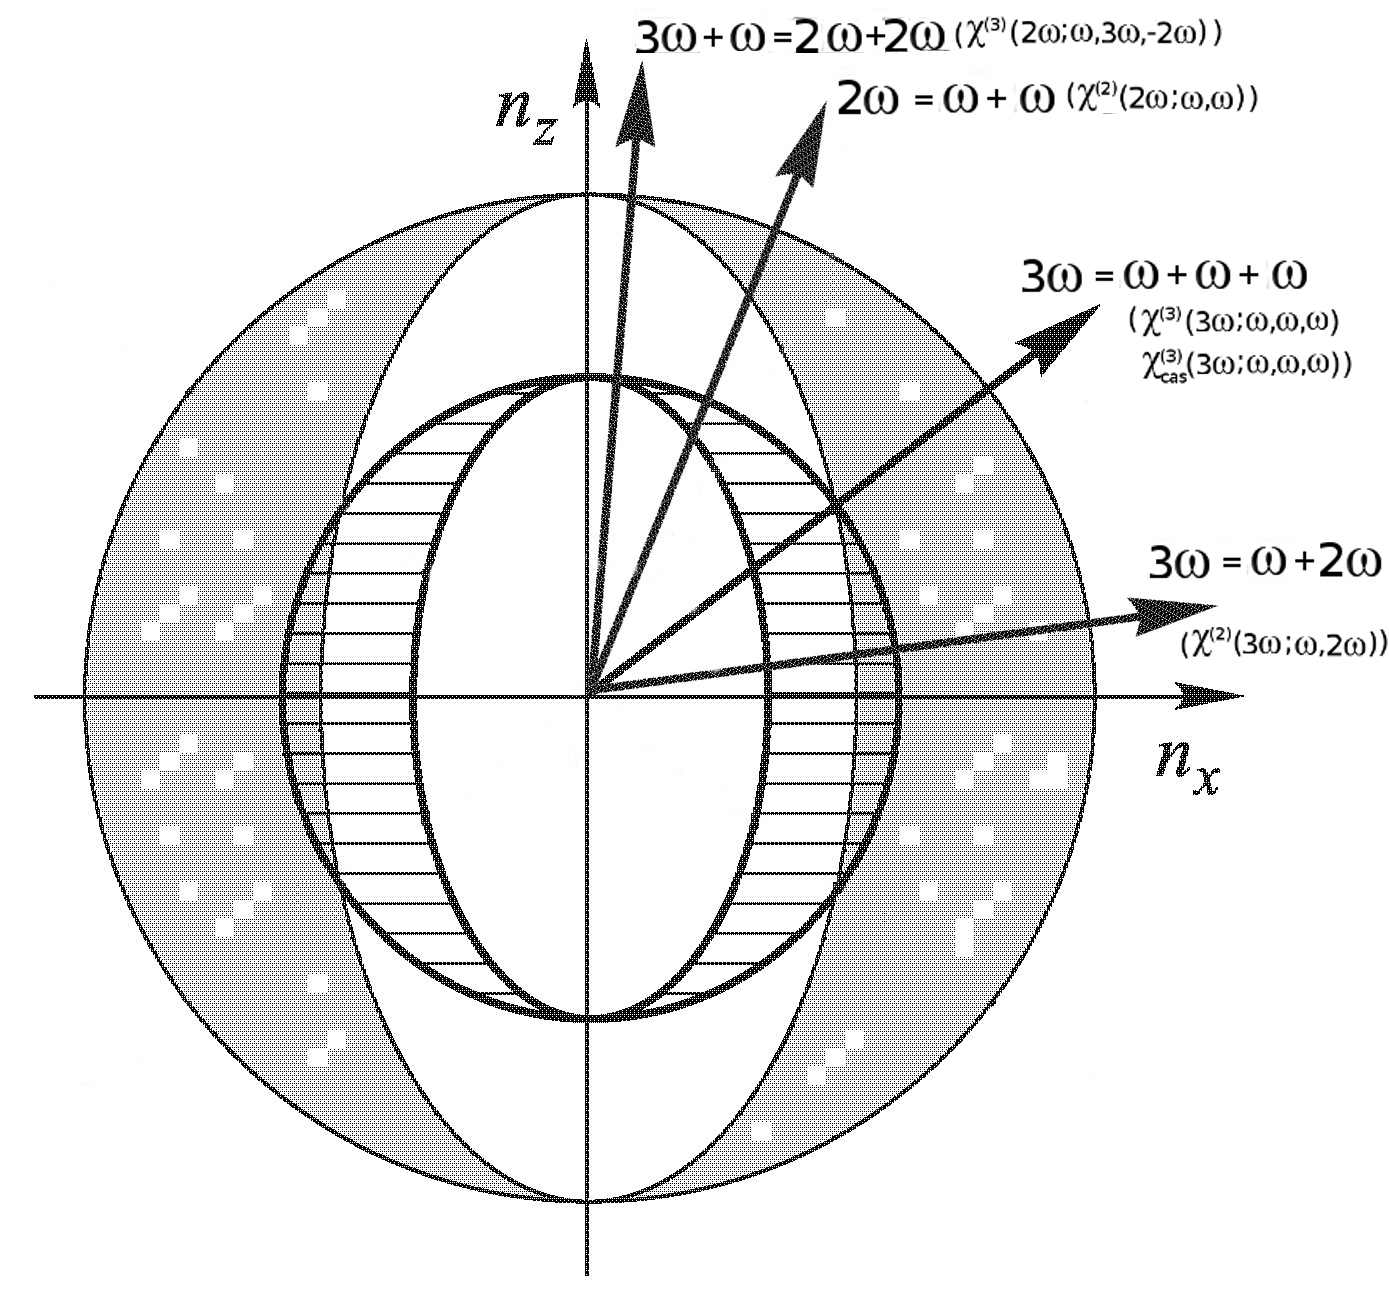
\includegraphics[width=0.4\textwidth]{Matching2}
\caption{Scheme of the phase matching and mismatching for various processes of frequency conversion.}
\label{fr:match}
\end{figure}
We suppose that the angle range for the achieving the phase matching of the corresponding generation process is small enough to avoid its overlapping with phase matching angle range of other processes. In this case, it is possible to differ the process of THG, which occurs due to the SFG process, and due to the cascading SHG.

Starting from Maxwell's equations it is easy to see that the optical frequency tripling of the  high intense femtosecond pulse in the frame-work of the plane wave approximation (without taking into account a laser beam diffraction) is described by the following set of dimensionless Schr\"{o}dinger equations with respect to slowly varying envelopes of the wave packets:
\begin{equation}
\label{eq:ref1}
\begin{aligned}
&L_jA_j+i\frac{\partial F}{\partial A_j^*}+iF_{selj}(A_1,\,A_2,\,A_3)=0,\,0< z \leq L_z , 0<t<L_t,\\
&L_j=\frac{\partial}{\partial z}+\nu_{j1}\frac{\partial}{\partial t}+iD_j\frac{\partial^2}{\partial t^2},\\
&F=\gamma_1({A_1^*}^2A_2e^{-i\Delta_{21} kz}+A_1^2A_2^*e^{i\Delta_{21} kz})+\gamma_2 (A_1^*A_2^* A_3e^{-i(\Delta_{31}k-\Delta_{21}k)z}\\
+&A_1A_2A_3^*e^{i(\Delta_{31}k-\Delta_{21}k)z})+\alpha_1({A_1^*}^3 A_3 e^{-i\Delta_{31}kz}+A_1^3 A_3^* e^{i\Delta_{31}kz})\\
+&\alpha_2(A_1^*A_2^2 A_3^*e^{-i(2\Delta_{21}k-\Delta_{31}k )z}+A_1{A_2^*}^2 A_3e^{i(2\Delta_{21}k-\Delta_{31}k )z}),\\
&F_{selj}=j\alpha_3 A_j(2\sum\limits_{k=1}^3 |A_k|^2-|A_j|^2), j=1,\,2,\,3, \nu_{11}=0.\\
\end{aligned}
\end{equation}
Here \(A_1,\,A_2\) and \(A_3\) are the complex amplitudes of waves with the basic frequency (\(\omega\)), and the doubled frequency (\(2\omega\)), and the tripled frequency (\(3\omega\)), respectively, normalized at \(A_{01}=\sqrt{I_{01}}\) (a square root of the maximal intensity of the incident pulse at the FF). Parameter \(\gamma_j\) is a coefficient of nonlinear coupling of the interacting waves due to the quadratic nonlinear response at the corresponding frequencies. In general case, this coefficient may be different for various generation processes. However, for simplicity, we choose the same value (\(\gamma_j=\gamma\)) for all these processes involving in equations \eqref{eq:ref1}. Parameters \(\alpha_j\) characterize the cubic nonlinear response of a medium at corresponding frequencies. Its influence results in the self-modulation and cross-modulation of the interacting waves as well as in the THG process. Further, for simplicity, we will suppose that all coefficients \(\alpha_j\) are also the same: \(\alpha_j=\alpha\). Parameter \(\Delta_{21} k=k_2 - 2k_1\)  characterizes the phase mismatching on the length $Z_n=1\,mm$, in which units a longitudinal coordinate $z$ is measured at the SHG. \(k_1\) and \(k_2\) denote dimensionless wavenumbers for waves with the FF and doubled frequency. Parameter \(\Delta_{31} k=k_3 - 3k_1\) characterizes the phase mismatching on $Z_n$ at THG. \(k_3\) denotes dimensionless TH wavenumber. Coordinate \(t\) is a time, measured in units of the pulse duration \(\tau_P\) at the FF. Parameters \(\nu_{21}\) and \(\nu_{31}\) characterize dimensionless GVM between SH and FW, and TH and FW, respectively. Parameters \(D_{j}, j=1,2,3\) characterize dimensionless SOD of the corresponding wave packet. Parameters \(L_t\) and \(L_z\) define the time interval, during which the laser pulse interaction is analyzed, and the maximal distance of the pulse propagation, respectively.

The initial distributions of the complex amplitudes are the following:
\begin{equation}\begin{aligned}
\label{eq:first}
&A_1(0,t)=A_{10}(t),\, A_2(0,t)=0,\,A_3(0,t)=0,\, t\in[0,L_t],\\
\end{aligned}\end{equation}
and corresponds to a finite distribution of the laser pulses.

Let us discuss the terms in the set of the equations \eqref{eq:ref1}. The term \(\gamma_1 A_1^2e^{i\Delta_{21} kz}\) (\(\chi^{(2)}(2\omega;\,\omega,\omega\))) in the second equation corresponds to the generation of a wave with doubled frequency for the process (\(\omega+\omega\rightarrow2\omega\)). The term \(\gamma_1  A_1^* A_2e^{-i\Delta_{21} kz}\) in the first equation is responsible for the opposite process (\(2\omega \rightarrow \omega+\omega\)). The term \(\alpha_1 A_1^3e^{i\Delta_{31}kz}\) (\(\chi^{(3)}(3\omega;\,\omega,\omega,\omega\))) in the third equation corresponds to THG due to cubic nonlinear response, and the term \(\alpha_1 {A_1^*}^2 A_3 e^{-i\Delta_{31}kz}\) in the first equation corresponds to the opposite process (\(3\omega\rightarrow\omega+\omega+\omega\)). A process of the THG via the SFG is described by the term \(\gamma_2 A_1 A_2e^{i(\Delta_{31}k-\Delta_{21}k)z}\) (\(\chi^{(2)}(3\omega;\,\omega,2\omega\))) in the third equation. The term \(\gamma_2 A_2^* A_3e^{-i(\Delta_{31}k-\Delta_{21}k)z}\) in the first equation the term \(\gamma A_1^* A_3e^{-i(\Delta_{31}k-\Delta_{21}k)z}\) in the second equation correspond to the reverse processes (\(3\omega\rightarrow2\omega+\omega\)). The phase mismatching for this process (denoted as \(\Delta_{SFG}k\)) is expressed through the phase mismatching of SHG and THG processes: \(\Delta_{SFG}k=\Delta_{31}k-\Delta_{21}k\). The terms \(\alpha_3 A_j|A_j|^2, j=1,\,2,\,3\) and \(\alpha_3 A_j|A_k|^2,\,j=1,2,3,\,k=1,2,3,j\ne k\) are responsible for the self- and the cross-modulation of waves, respectively. SHG via the process (\(3\omega+\omega\rightarrow2\omega+2\omega\)) corresponds to the term \(\alpha_2 A_1A_2^*A_3e^{i(2\Delta_{21}k-\Delta_{31}k )z}\) (\(\chi^{(3)}(2\omega;\,\omega,3\omega,-2\omega\))) in the second equation, and the term \(\alpha_2 A_2^2 A_3^*e^{-i(2\Delta_{21}k-\Delta_{31}k )z}\) in the first equation and the term \(\alpha_2 A_1^* A_2^2 e^{-i(2\Delta_{21}k-\Delta_{31}k )z}\) in the third equation correspond to the opposite process (\(2\omega+2\omega\rightarrow3\omega+\omega\)). In this case, the phase mismatching is the following: \(\Delta_{WM}k=2\Delta_{21}k-\Delta_{31}k\).

 Let us note that the introduced dimensionless parameters and functions are expressed through the physical ones, denoted with containing line above them, with accordance to a rule:
\begin{equation}
\label{eq:pars}
\begin{aligned}
&A_j=\frac{\bar{A}_j}{\sqrt{I_{01}}},\,D_j=-\frac{1}{2}\frac{\partial^2 \bar{k}}{\partial \bar{\omega}^2}\Big|_{\bar{\omega}_j}\frac{Z_n}{\tau_P^2},\omega_j=\bar{\omega}_j\tau_P,\,j=1,2,3,\,t=\frac{\bar{t}}{\tau_P},\,z=\frac{\bar{z}}{Z_n},\\
&\nu_{j1}=\left(\frac{\partial \bar{k}}{\partial \bar{\omega}}\Big|_{j\bar{\omega}}-\frac{\partial \bar{k}}{\partial \bar{\omega}}\Big|_{\bar{\omega}}\right)\frac{Z_n}{\tau_P},\,\Delta_{j1}k=\Delta_{j1}\bar{k}Z_n,\,j=2,\,3\\
&\gamma=\frac{2\pi\chi^{(2)}\bar{k}\sqrt{I_{01}}}{n^2}Z_n,\,\alpha=\frac{3\pi \bar{k}}{2n^2}\chi^{(3)}I_{01} Z_n,
\end{aligned}
\end{equation}
$n$ is a refractive index with FF. For computer simulation we choose the following values of the physical parameters: \(\tau_P \text{ is changed from } 100fs\text{ to }10ps,\) the wavelength corresponding to wave with FF is equal to \(\lambda_1=1064\,nm\) or \(\lambda_1=800\,nm\). We give the linear and nonlinear characteristics of some nonlinear crystals in Methods.
\textcolor{ForestGreen}{\section{THG in a medium with quadratic nonlinear response}}
\subsection{Equations, describing THG in a medium with quadratic nonlinear response}
To derive the equations, containing induced cubic response under the condition of the cascading SHG, we use multiscale method \cite{bib:n24}, which was applied in \cite{bib:n19} for the deriving of the equation, describing the pulse self-compression (decompression) under the same process. Because our current interest lies in demonstration of the THG in a medium with the quadratic nonlinear response we consider a case \(\alpha=0\) \textcolor{blue}{and \(\Delta_{31}k=0\), which corresponds to the phase matching between the incident wave and the wave with treble frequency}. Therefore, in equations \eqref{eq:ref1} we omit the terms with cubic nonlinear response.

\textcolor{blue}{Here we derive the equation set \eqref{eq:main} which describes a THG process at } \textcolor{ForestGreen}{Then, we consider} big phase mismatching between SH and FW: \(|\Delta_{21}k|>>1\). In this case, the process of wave interaction possesses various space scales: in particular, a small scale, defined by big phase mismatching \(|\Delta_{21}k|\), and a long space scale defined by the dispersion lengths of the interacting pulses. 

\textcolor{ForestGreen}{
First of all, we make a substitution of TH complex amplitude, which involve only its phase:
$$
\bar{A}_3=A_3e^{i\Delta_{31}kz},
$$
(this bar is omitted below for brevity). This is made for simplicity of further analysis, and the equation set \eqref{eq:ref1} takes the form
\begin{equation}
\label{eq:refg}
\begin{aligned}
&\frac{\partial{A_1}}{\partial{z}}+iD_1\frac{\partial^2{A_1}}{\partial{t^2}}+i\gamma\left(A_1^* A_2e^{-i\Delta_{21} kz}+A_2^* A_3e^{i\Delta_{21}kz}\right)=0,\\
&\frac{\partial{A_2}}{\partial{z}}+\nu_{21}\frac{\partial A_2}{\partial t}+iD_2\frac{\partial^2{A_2}}{\partial{t^2}}+i\gamma\left(A_1^2e^{i\Delta_{21} kz}+2A_1^*A_3e^{i\Delta_{21}kz}\right)=0,\\
&\frac{\partial{A_3}}{\partial{z}}+\nu_{31}\frac{\partial A_3}{\partial t}+iD_3\frac{\partial^2{A_3}}{\partial{t^2}}+3i\gamma A_1 A_2e^{-i\Delta_{21}kz}+i\Delta_{31}kA_3=0,\,0< z \leq L_z , 0<t<L_t.\\
\end{aligned}\end{equation}
}

Let us introduce a small parameter \(\mu=\frac{1}{\Delta_{21}k}\) (for simplicity, we suppose that the phase mismatching has a positive sign) and introduce various scales along \(z\) coordinate: small scale equal to the inverse phase mismatching length: \(\xi=\frac{z}{\mu}\), and big longitudinal scales \(z_l=\mu^lz,\,l=0,1,2...\). Because of the big absolute value of the phase mismatching, the SHG efficiency is very low. Therefore, the complex amplitudes are expanded in a power series of \(\mu\):
\begin{equation}
\label{eq:exp}
\begin{aligned}
&A_1=U+\mu U_1 +\mu^2 U_2 +...,\\
&A_2=V+\mu V_1 + \mu^2 V_2 +...,\\
&A_3=W+\mu W_1 + \mu^2 W_2+....\\
\end{aligned}
\end{equation}
Obviously, the functions in \eqref{eq:exp} depend on all the variables \((t,\xi,z_l|l\ge0)\).

Using the chain rule, we write differential operators in terms of new variables:
\begin{equation}
\label{eq:op}
\begin{aligned}
L_j&=\frac{\partial}{\partial z}+\nu_{j1}\frac{\partial}{\partial t}+iD_j\frac{\partial^2}{\partial t^2}=\frac{\partial \xi}{\partial z}\frac{\partial}{\partial \xi}+\sum\limits_{l=0}^{\infty}\frac{\partial z_l}{\partial z}\frac{\partial}{\partial z_l}+iD_j\frac{\partial^2}{\partial t^2}=\frac{1}{\mu}\frac{\partial}{\partial \xi}+\sum\limits_{l=0}^{\infty} \mu^l\frac{\partial}{\partial z_l}+iD_j\frac{\partial^2}{\partial t^2}\\
&=\frac{1}{\mu}\frac{\partial}{\partial \xi}+L_j^{0}+\mu\frac{\partial}{\partial z_1}+\mu^2 \frac{\partial}{\partial z_2}+...,j=1,2,3.
\end{aligned}
\end{equation}
Here, operator \(L_j\) is defined as 
\[L_j^{(0)}=\frac{\partial}{\partial z_0}+\nu_{j1}\frac{\partial}{\partial t}+ iD_j\frac{\partial^2}{\partial t^2}.\]

Then, we substitute the expansion \eqref{eq:exp} into the equation set \eqref{eq:refg}. For brevity, we write only the term \(A_1^*A_2\):
\[A_1^*A_2=\left(U^*+\mu U_1^*+O(\mu^2)\right)\left(V+\mu V_1+O(\mu^2)\right)=U^*V+\mu\left(U^*V_1+U_1^*V\right)+O(\mu^2).\]  
Providing similar math operations for other terms, we write all terms with an order, which is greater than \(\mu^2\):
\begin{equation}
\label{eq:allset}
\begin{aligned}
&\frac{1}{\mu}\frac{\partial U}{\partial \xi}+L_1^{(0)}U+\mu \frac{\partial U}{\partial z_1}+\frac{\partial U_1}{\partial\xi}+\mu L_1^{(0)}U_1+\mu\frac{\partial U_2}{\partial \xi}+\\
+&i\gamma\left(U^*Ve^{-i\xi}+V^*We^{i\xi}+\mu((U^*V_1+U_1^*V)e^{-i\xi}+(V^*W_1+V_1^*W)e^{i\xi})\right)+O(\mu^2)=0,\\
&\frac{1}{\mu}\frac{\partial V}{\partial \xi}+L_2^{(0)}V+\mu \frac{\partial V}{\partial z_1}+\frac{\partial V_1}{\partial\xi}+\mu L_1^{(0)}V_1+\mu\frac{\partial V_2}{\partial \xi}+\\
+&i\gamma\left(U^2e^{i\xi}+2U^*We^{i\xi}+\mu(2UU_1e^{i\xi}+(U^*W_1+U_1^*W)e^{i\xi})\right)+O(\mu^2)=0,\\
&\frac{1}{\mu}\frac{\partial W}{\partial \xi}+L_3^{(0)}W+\mu \frac{\partial W}{\partial z_1}+\frac{\partial W_1}{\partial\xi}+\mu L_1^{(0)}W_1+\mu\frac{\partial W_2}{\partial \xi}+\\
+&3i\gamma \left(UVe^{-i\xi}+\mu(UV_1+U_1V)e^{-i\xi}\right)+i\Delta_{31}k(W+\mu W_1)+O(\mu^2)=0.
\end{aligned}
\end{equation}
Grouping the terms with respect to power of \(\mu\) we obtain the equations:
\[\frac{\partial U}{\partial \xi}=\frac{\partial V}{\partial \xi}=\frac{\partial W}{\partial \xi}=0,\]
corresponding to \(\frac{1}{\mu}\) power of the expansion. Consequently, the functions \(U,\,V\) and \(W\) do not depend on fast changing coordinate \(\xi\). Therefore, these functions do not change at the small scale.

For the next order \(O(1)\) of power \(\mu\), we obtain the following set of equations:
\begin{equation}
\label{eq:fo}
\begin{aligned}
&L_1^{(0)}U+\frac{\partial U_1}{\partial\xi}+i\gamma(U^*Ve^{-i\xi}+V^*We^{i\xi})=0,\\
&L_2^{(0)}V+\frac{\partial V_1}{\partial \xi}+i\gamma(U^2e^{i\xi}+2U^*We^{i\xi})=0,\\
&L_3^{(0)}W+\frac{\partial W_1}{\partial \xi}+3i\gamma UVe^{-i\xi}+i\Delta_{31}kW=0.\\
\end{aligned}
\end{equation}
So, since the first terms in these equations do not depend on \(\xi\), meanwhile other terms do depend on this variable, we can separate equations into two parts. The first of them is written as
\begin{equation}
\label{eq:m1}
L_1^{(0)}U=L_2^{(0)}V=L_3^{(0)}W+i\Delta_{31}kW=0.
\end{equation}
The functions \(U_1,\,V_1,\,W_1\) can be found from the second one by integrating \eqref{eq:fo} with respect to \(\xi\):
\begin{equation}
\label{eq:ford}
\begin{aligned}
&U_1=\gamma(U^*Ve^{-i\xi}-V^*We^{i\xi})+u_1(t,z_0,\,z_1...),\\
&V_1=\gamma(-U^2e^{i\xi}-2U^*We^{i\xi})+v_1(t,z_0,\,z_1...),\\
&W_1=3\gamma UVe^{-i\xi}+w_1(t,z_0,\,z_1...).\\
\end{aligned}
\end{equation}
Here \(u_1, v_1, w_1\) are the function of integration: they do not depend on \(\xi\). The equations, which they are governed by, are derived further.

At the order \(O(\mu)\), the equations are the following:
\[\begin{aligned}
&\frac{\partial U_2}{\partial \xi}+L_1^{(0)}U_1+\frac{\partial U}{\partial z_1}+i\gamma((U^*V_1+U_1^*V)e^{-i\xi}+(V^*W_1+V_1^*W)e^{i\xi})=0,\\
&\frac{\partial V_2}{\partial \xi}+L_2^{(0)}V_1+\frac{\partial V}{\partial z_1}+i\gamma(2UU_1e^{i\xi}+(U^*W_1+U_1^*W)e^{i\xi})=0,\\
&\frac{\partial W_2}{\partial \xi}+L_3^{(0)}W_1+\frac{\partial W}{\partial z_1}+3i\gamma(UV_1+U_1V)e^{-i\xi}+\Delta_{31}kW_1=0.\\
\end{aligned}\]

Using the representation \eqref{eq:ford} this set transforms into the form:
\begin{small}
\[\begin{aligned}
&\frac{\partial U_2}{\partial \xi}+\gamma(L_1^{(0)}(U^*V)e^{-i\xi}-L_1^{(0)}(V^*W)e^{i\xi})+i\gamma^2(U^*v_1e^{-i\xi}-V^2W^*e^{-2i\xi}+u_1^*Ve^{-i\xi}+V^*w_1e^{i\xi}+v_1^*We^{i\xi})=\\
&-\left(\frac{\partial U}{\partial z_1}+i\gamma^2(-|U|^2U-3U^{*2}W+4U|V|^2-2U|W|^2)\right)-L_1^{(0)}u_1,\\
&\frac{\partial V_2}{\partial \xi}-\gamma(L_2^{(0)}(U^2)e^{i\xi}+2L_2^{(0)}(U^*W)e^{i\xi})+i\gamma^2(-2UV^*We^{2i\xi}+2Uu_1e^{i\xi}+2UV^*We^{i\xi}+2u_1^*We^{i\xi}+2U^*we^{i\xi})=\\
&-\left(\frac{\partial V}{\partial z_1}+2i\gamma^2(4|U|-|W|^2)V\right)-L_2^{(0)}v_1,\\
&\frac{\partial W_2}{\partial \xi}+3\gamma L_3^{(0)}(UV)e^{-i\xi}+3i\gamma^2(Uv_1e^{-i\xi}+U^*V^2*e^{-2i\xi}+u_1V_1e^{-i\xi})+3i\Delta_{31}k\gamma UVe^{-i\xi}=\\
&-\left(\frac{\partial W}{\partial z_1}-3i\gamma^2(U^3+2|U|^2W+|V|^2W)\right)-L_1^{(0)}w_1-i\Delta_{31}kw_1.\\
\end{aligned}\]
\end{small}
As before, we can state that the right-hand sides of the equations are equal to zero because they do not depend on \(\xi\) in contrast to the left-hand sides of the equations. Thus, we write the equations
\[\begin{aligned}
&\frac{\partial U}{\partial z_1}+i\gamma^2(-|U|^2U-3U^{*2}W+4U|V|^2-2U|W|^2)=-L_1^{(0)}u_1,\\
&\frac{\partial V}{\partial z_1}+2i\gamma^2(4|U|^2-|W|^2)V=L_2^{(0)}v_1,\\
&\frac{\partial W}{\partial z_1}-3i\gamma^2(U^3+2|U|^2W+|V|^2W)=L_3^{(0)}w_1+i\Delta_{31}kw_1.\\
\end{aligned}\]
Here, we separate terms, which contain \(u_1,\,v_1,\,w_1\). Since in the representation \eqref{eq:exp} they belong to order \(O(\mu)\), meanwhile, \(U,\,V,\,W\) belong to order \(O(1)\), then we can once again separate the obtained equation into two parts: 
\begin{equation}
\label{eq:mai}
\begin{aligned}
&\frac{\partial U}{\partial z_1}+i\gamma^2(-|U|^2U-3U^{*2}W+4U|V|^2-2U|W|^2)=0,\\
&\frac{\partial V}{\partial z_1}+2i\gamma^2(4|U|^2-|W|^2)V=0,\\
&\frac{\partial W}{\partial z_1}-3i\gamma^2(U^3+2|U|^2W+|V|^2W)=0.\\
\end{aligned}
\end{equation}
 Consequently, the equations
\begin{equation}
\begin{aligned}
&L_1^{(0)}u_1=0,\\
&L_2^{(0)}v_1=0,\\
&L_3^{(0)}w_1+i\Delta_{31}kw_1=0\\
\end{aligned}
\end{equation}
are valid.

After returning to original variables (\(\xi=\Delta_{21}kz,\,z_0=z,\,z_1=z/\Delta_{21}k,\,\frac{\partial}{\partial z}=\Delta_{21}k\frac{\partial}{\partial \xi}+\frac{\partial}{\partial z_0}+\frac{1}{\Delta_{21}k}\frac{\partial}{\partial z_1}+O(\Delta_{21}k^{-2})\)), we obtain the following set of equations:
\begin{equation}
\label{eq:main}
\begin{aligned}
&\frac{\partial U}{\partial z}+iD_1\frac{\partial^2 U}{\partial t^2}-i\frac{\gamma^2}{\Delta_{21} k}(|U|^2U+3U^{*2}W-4U|V|^2+2U|W|^2)=0,\\
&\frac{\partial V}{\partial z}+\nu_{21}\frac{\partial V}{\partial t}+iD_2\frac{\partial^2 V}{\partial t^2}+2i\frac{\gamma^2}{\Delta_{21} k}(4|U|^2-|W|^2)V=0,\\
&\frac{\partial W}{\partial z}+\nu_{31}\frac{\partial W}{\partial t}+iD_3\frac{\partial^2 W}{\partial t^2}-3i\frac{\gamma^2}{\Delta_{21} k}(U^3+2|U|^2W+|V|^2W)+i\Delta_{31}kW=0\\
\end{aligned}
\end{equation}
with respect to \(U,V,W\), and the functions \(u_1,v_1,w_1\) are the solution of the linear Schr\"{o}dinger equations:
\begin{equation}
\label{eq:main_2}
\begin{aligned}
&\frac{\partial u_1}{\partial z}+iD_1\frac{\partial^2 u_1}{\partial t^2}=0,\\
&\frac{\partial v_1}{\partial z}+\nu_{21}\frac{\partial v_1}{\partial t}+iD_2\frac{\partial^2 v_1}{\partial t^2}=0,\\
&\frac{\partial w_1}{\partial z}+\nu_{31}\frac{\partial w_1}{\partial t}+iD_3\frac{\partial^2 w_1}{\partial t^2}+i\Delta_{31}kw_1=0.\\
\end{aligned}
\end{equation}
The expansion series \eqref{eq:exp} transforms into the following form:
\begin{equation}
\label{eq:exp2}
\begin{aligned}
&A_1=U+\frac{1}{\Delta_{21}k}\left(\gamma(U^*Ve^{-i\Delta_{21}kz}-V^*We^{i\Delta_{21}kz})+u_1\right),\\
&A_2=V+\frac{1}{\Delta_{21}k}\left(-\gamma(U^2+2U^*W)e^{i\Delta_{21}kz}+v_1\right),\\
&A_3=W+\frac{1}{\Delta_{21}k}\left(3\gamma UVe^{-i\Delta_{21}kz}+w_1\right).\\
\end{aligned}
\end{equation}
Let us note that if we do not take into account the THG process (\(A_3=W=w_1=0\)), then the equations \eqref{eq:exp2}-\eqref{eq:main} reduce to the corresponding ones, derived in \cite{bib:n19}.

In accordance with our aim, we consider below a special case of a frequency conversion: the absence of SH and TH in the input section of a medium. It means that the complex amplitudes \(A_2\) and \(A_3\) are equal to zero in this section. Therefore, at the definition of the initial conditions for the functions \(U,\,V,\,W\) and \(u_1,\,v_1,\,w_1\), we also compare the corresponding terms in a series with respect to the small parameter \((\Delta_{21}k)^{-1}\) in \eqref{eq:exp2}. Thus, the main terms \(V\) and \(W\) in the representation \eqref{eq:exp2} equal zero while \(U\) has the same initial distribution as \(A_1\) (see \eqref{eq:first}):
\[
\begin{aligned}
&U|_{z=0}=A_1|_{z=0}=A_{10}(t),\\
&V|_{z=0}=A_2|_{z=0}=0,\\
&W|_{z=0}=A_3|_{z=0}=0.\\
\end{aligned}
\]
Since the initial distributions of the complex amplitudes \(A_j,\,j=1,2,3\) do not contain the terms at \((\Delta_{21}k)^{-1}\), then the corresponding terms in \eqref{eq:exp2} should be chosen equal to zero:
\[
\begin{aligned}
&\gamma\left(U^*|_{z=0}V|_{z=0}-V^*|_{z=0}W|_{z=0}\right)+u_1|_{z=0}=0,\\
&\gamma\left(-U^2|_{z=0}-2U^*|_{z=0}W|_{z=0}\right)+v_1|_{z=0}=0,\\
&3\gamma U|_{z=0}V|_{z=0}+w_1|_{z=0}=0.\\
\end{aligned}
\]
Solving these equations, we obtain the following initial conditions:
\begin{equation}
\label{eq:ini3}
U|_{z=0}=A_{10}(t),\, V|_{z=0}=W|_{z=0}=0,\, u_1|_{z=0}=w_1|_{z=0}=0,\, v_1|_{z=0}=\gamma A_{10}^2(t)
\end{equation}
for the sets of equations \eqref{eq:main}, \eqref{eq:main_2}. 

Then the equations sets \eqref{eq:main}, \eqref{eq:main_2} reduce to the following view:
\textcolor{blue}{The detail derivation of the modified equations is presented in Methods. Here we write only the resulting formulas for the complex amplitudes taking into account the first order of the parameter \(1/\Delta_{21}k\) at power series expansion:} 
\begin{equation}
\label{eq:exp3}
\begin{aligned}
&A_1=U, A_2=\frac{1}{\Delta_{21}k}(-\gamma (U^2+2U^*W)e^{i\Delta_{21}kz}+v_1), A_3=W.\\
\end{aligned}
\end{equation}
Here functions \(U,\,W,\,v_1\) are governed by the set of nonlinear equations:
\begin{equation}
\label{eq:main2}
\begin{aligned}
&L_1U-i\frac{\gamma^2}{\Delta_{21} k}(|U|^2U+3U^{*2}W+2U|W|^2)=0,\\
&L_3W-3i\frac{\gamma^2}{\Delta_{21} k}(U^3+2|U|^2W)+i\Delta_{31}kW=0,\,L_2 v_1=0.\\
\end{aligned}
\end{equation}
because \(V\equiv0\) due to the initial conditions \eqref{eq:ini3} and containing of the function \(V\) in all terms belonging to the second equation of the equations set \eqref{eq:main}, and a similar analysis shows that \(u_1\equiv0,\,w_1\equiv0\).

\textcolor{ForestGreen}{According to \eqref{eq:ini2}, these equations are supplemented} with the following initial conditions:
\begin{equation}
\label{eq:ini2}
U|_{z=0}=A_{10}(t),\,W|_{z=0}=0,\,v_1|_{z=0}=\gamma A_{10}^2(t).
\end{equation}
and zero-valued BCs because all pulses have finite initial distribution and we consider bounded domain in \(z\)-coordinate. We call below the problem \eqref{eq:main2}-\eqref{eq:ini2} as the modified problem.

\textcolor{ForestGreen}
{
\subsection{Cubic nature of induced nonlinear response}
}
We depict in Fig. \ref{fr:f}a a verification that in a medium with quadratic susceptibility, the cubic nonlinear response can be induced due to the cascading SHG. We show here the dependence of the TH intensity, and the THG efficiency on the incident pulse maximal intensity (this intensity changes between 1 and 4 dimensionless units) computed both in long pulse duration approximation (lines) and at remarkable SOD (\(D_1=-0.0032, D_2 =  -0.0083, D_3 =  -0.0199\), rounds and triangles, stars and squares) for two cases. In the first one, the pulses propagate in a medium with the quadratic susceptibility at \(\Delta_{21}k=20\). In the second one, we consider THG (SH is absent) in a medium with the cubic susceptibility at the appropriate choice of the parameter \(\alpha\) being equal to \(3\gamma^2/\Delta_{21}k\) \textcolor{ForestGreen}{(as it follows from the equations sets \eqref{eq:ref1},\eqref{eq:main}, in this case, both sets possess the same coefficient at $A_1^3$ (or $U^3$) in the equation with respect to the TH)}. We see that the pulse intensity and the frequency conversion efficiency changes in both cases practically in the same way. All these results show that the cascading SHG induces the cubic nonlinearity.
\begin{figure}[h!] 
\centering 
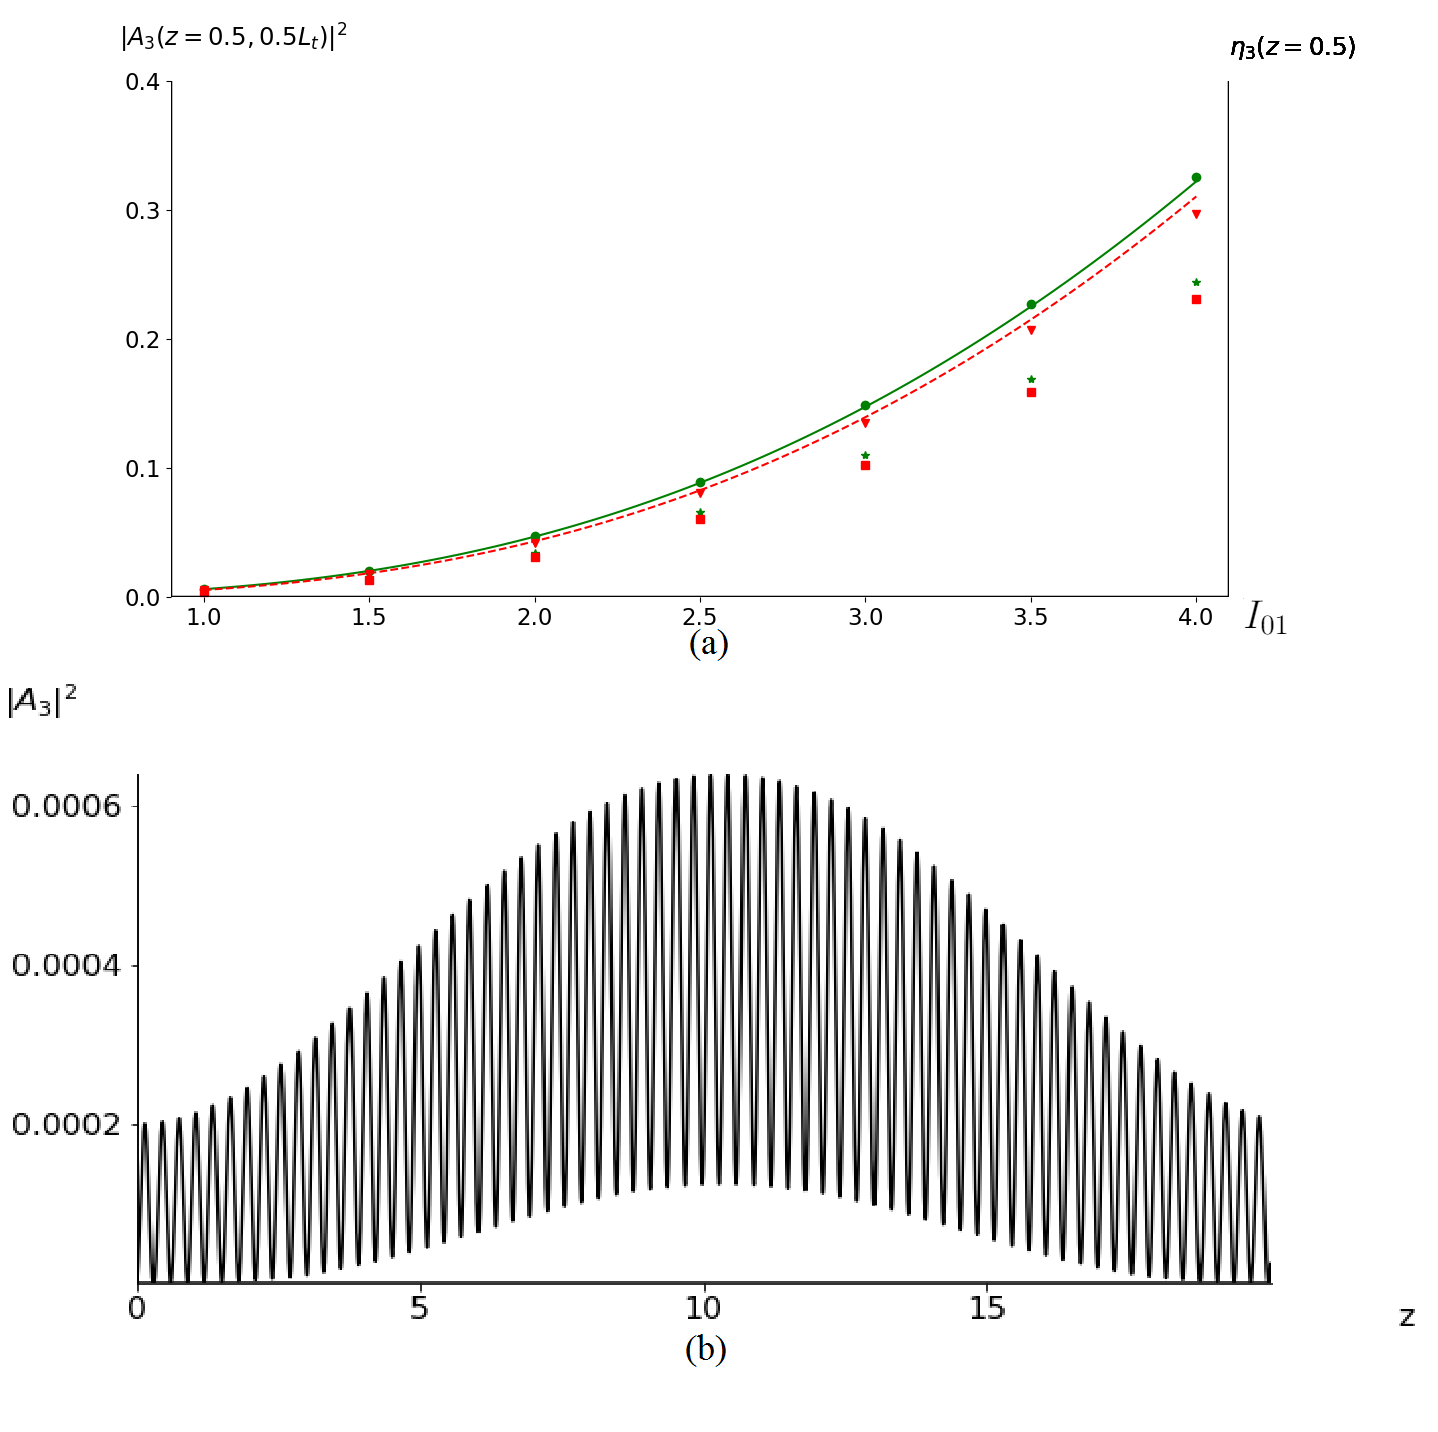
\includegraphics[height=10cm, width=0.7\linewidth]{CascadeF}  
\caption{TH maximal intensity dependence on the FW maximal incident intensity computed at parameters \(\gamma=1,\alpha=0,\Delta_{21}k=20,\,\Delta_{31}k=0\) (solid line, rounds and stars) and at \(\gamma=0,\alpha=0.15,\Delta_{21}k=0,\,\Delta_{31}k=0\) (dashed line, triangles and squares) under long pulse duration approximation (lines) and SOD influence (\(D_1=-0.0032, D_2 =  -0.0083, D_3 =  -0.0199\), rounds and triangles, stars and squares) (a). TH maximal intensity computed at $\gamma=1,\,\alpha=0.15,\Delta_{21}k=20,\,\Delta_{31}k=0,D_j=0,j=1,\,2,\,3$ (b)}
\label{fr:f}
\end{figure}

\textcolor{ForestGreen}
{
Another verification is obtained from the simulation of a THG in a medium with combined quadratic and cubic nonlinear response, where parameter $\alpha$ again equals to $3\gamma^2/\Delta_{31}k$, so, according to our theory, the cubic nonlinear response of a medium and the induced cubic nonlinear will compensate each other. As we see in Fig. \ref{fr:f}b, this indeed happens, since the TH maximal intensity does not exceed $0.0006$. We show below that much more promising results can be obtained. This result is obtained in long pulse duration approximation, so only nonlinear effects are considered, which, as we say, annihilate each other.  
}

\textcolor{ForestGreen}
{
\subsection{Influence of phase mismatchings on the THG efficiency}
It should be stressed that the modified problem can be solved analytically in long pulse duration approximation, when SOD effects are negligibly small $|D_j|<<1$. The formulas, describing TH intensity evolution, are derived in Methods, here we present the main results. The major characteristics (such as TH intensity maximum and the crystal length, required for this intensity achievement) depend on the ratio of problem parameters
$$
p=\frac{\Delta_{21}k\Delta_{31}k}{\gamma^2}.
$$
The theory predicts that the THG maximal possible efficiency of more than $95\%$ is achieved at $p=3+ \frac{9}{\sqrt[3]{2}}-9\sqrt[3]{2}\approx-1.2$, as one can see in Fig. \ref{fr:cglp}a,
\begin{figure}
    \centering
    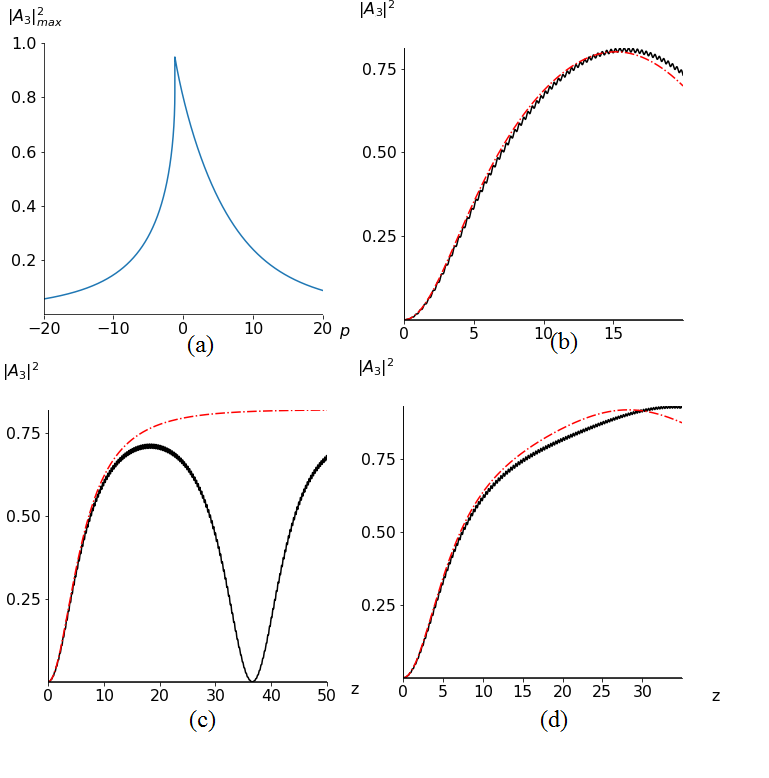
\includegraphics[width=0.8\textwidth, height=0.4\textheight]{CGLP.png}
    \caption{TH intensity maximum with respect to the parameter p (a). TH intensity along $z$--coordinate for the original (black solid line) and modified (red dashed-dotted line) problems computed at $\gamma=1,\Delta_{21}k=20,\,D_j=0,\,j=1,\,2,\,3$ and $\Delta_{31}k=0$ (b), $-0.0598$ (c), $-0.05$ (d)}
    \label{fr:cglp}
\end{figure}
and this means that the phase matching between TH and FW is not the optimal condition, because at $\Delta_{31}k=0$ (and, therefore, at $p=0$), only $80\%$ conversion efficiency can be achieved (which is also a very decent result). Another (not so surprising though) result from Fig. \ref{fr:cglp}a is that the TH intensity maximum is sufficiently lower for $|p|>>1$, i.e. at the same incident intensity, but greater $|\Delta_{21}k|$, the smaller interval of $\Delta_{31}k$ provides the remarakable THG. 
}  

\textcolor{ForestGreen}
{
However, this results are obtained for the modified problem, so they must be verified by the computer simulation of the original problem, which we also present here. First of all, we show that the conversion efficiency of $80\%$ is indeed achieved at phase matching between TH and FW approximately in the section $z=15$ (Fig. \ref{fr:cglp}b), and we see a good coincidence between solutions of both problems. In contrast to this, the contradiction between two solutions is observed in Fig. \ref{fr:cglp}c) at theoretically best case $p=3+ \frac{9}{\sqrt[3]{2}}-9\sqrt[3]{2}$, and only $|A_3|^2=0.7$ is achieved. The reason is that this parameter value is a border between two different areas of intensity evolution (see Methods for more details), so in this case the tiny factors (of order $O(\Delta_{21}k^{-2})$ and lower), which were neglected at derivation of the modified problem, play more important role than in other cases. Fortunately, if we slightly shift the parameter $\Delta_{31}k$ towards zero ($\Delta_{31}k=-0.05$ for definiteness), than the THG efficiency sufficiently improves and achieves the value of $93\%$ (Fig. \ref{fr:cglp}d).
}

\textcolor{ForestGreen}
{
Thus, we see that the phase matching is not necessary the best choice. It can be explained by analyzing of the set of the equations \eqref{eq:main2}. We see that the equation with respect to $W$ does not contain the self-modulation term $|W|^2W$, therefore, it is not symmetrical in contrast to the classical model of THG in a medium with cubic nonlinear response, so non-zero phase mismatching between FW and TH partly compensate FW self-modulation and cross-modulation between waves.
}

\textcolor{blue}
{
Another remark refers to the analytical solution of the problem \eqref{eq:main2}-\eqref{eq:ini2}. If the incident pulse duration is big enough to neglect SOD and GVM influence, then one can consider the problem in the framework of the long pulse duration approximation. In this case, the TH intensity depends only on \(z\)--coordinate, and it is expressed through the elliptical cosine:
\begin{equation}
\label{eq:sol}
p_3(z)=|A_3(z)|^2=\frac{4(1-cn(\frac{3\sqrt[4]{5}\gamma^2}{\Delta_{21}k}z; 0.5(1-\frac{1}{\sqrt{5}})))}{(5+\sqrt{5})-(5-\sqrt{5})cn(\frac{3\sqrt[4]{5}\gamma^2}{\Delta_{21}k}z; 0.5(1-\frac{1}{\sqrt{5}}))}.
\end{equation}
The derivation of this formula is made in Methods. Moreover, we find out also the TH phase evolution. Because of the complexity of the obtained formula, we do not write it here. However, using the formulas with respect to the phase and the intensity, it is possible to approximate the solution of the problem \eqref{eq:ref1}-\eqref{eq:first} with good accuracy. We show it below using the computer simulation results.
}

\textcolor{blue}{
For practice, it is very important to stress that, as follows from \eqref{eq:sol}, the problem parameters \(\gamma\) and \(\Delta_{21}k\) influence only on the intensity oscillation period: the TH maximal intensity remains the same for any values of these parameters and equals \(0.8\).
}
%\clearpage
\textcolor{blue}{
\section*{Computer simulation of the frequency tripling.}
}
\textcolor{ForestGreen}
{
\section{SOD influence on the frequency tripling}
}
Below we discuss the computer simulation results for the frequency tripling of the optical pulses and at phase matching of THG (\(\Delta_{31}k=0\)), and taking into account the SOD influence, and the group velocity matching: \(\nu_{21}=\nu_{31}=0\). We provide a computer simulation using the set of equations \eqref{eq:ref1} and the set of equations \eqref{eq:main2}. Our aim is a demonstration of the high efficient THG with a smooth shape of a pulse at the trebled frequency and its smooth spectrum. 

The incident pulse at the FF possesses Gaussian distribution without any chirp:
\begin{equation}
A_{10}(t)=A_{01}e^{-(t-0.5L_t)^2},
\end{equation}
where \(A_{01}\) is equal to unity due to chosen dimensionless parameters. However, the parameter \(A_{01}\) will be used in the Conclusion of the paper for the final illustration of the frequency conversion efficiency dependence on the incident pulse intensity.

It should be emphasized that below in paragraphs \ref{par:nor} and \ref{par:an} the solution of the problem \eqref{eq:ref1}-\eqref{eq:first} is depicted as a solid line while the solution of the modified problem  \eqref{eq:main2}-\eqref{eq:ini2} is shown as a dotted line.  Numbers \(1,\,2,\,3\) in the Figs. denote FW, SH, and TH, respectively. In some cases, we also demonstrate the applicability of the analytical solution derived in the long pulse duration approximation and this solution is depicted as a dashed line. We pay an attention to the pulses spectra and depict the initial spectrum distributions (as well as the FW initial pulse shape) in some Figs. via the solid line with triangles.

\subsection{Normal dispersion of a medium at FW wavelength}
\label{par:nor}
First of all, we consider the frequency tripling of the pulse with wavelength \(\lambda=800\,nm\) and propagating in a BBO crystal with the normal dispersion, which corresponds in our notations to negative values of the dimensionless SOD coefficients. In Fig. \ref{fr:c1_1}a-c the pulse shapes are depicted for the frequency upconversion at a relatively small phase mismatching between SH and FW (\(\Delta_{21}k=20\)) and at the incident pulse duration being about \(100fs\). It should be stressed that a positive sign of phase mismatching \(\Delta_{21}k\) corresponds to the FW pulse compression under its propagation in a medium with the normal SOD if the THG is not essential.

We see a good coincidence between the FW and TH pulse shapes, computed on using the original problem solution and the modified one, until the section \(z=13\). Despite a medium possesses only the quadratic nonlinearity (\(\alpha=0\)), the TH intensity is high: it achieves \(0.75\) dimensionless units at the pulse center. This growth accompanies by the spectral broadening of the FW and TH pulses in comparison with the incident FW pulse spectrum. However, the FW pulse spectrum has two local minimums in this section of a medium. 

After the distance equals 10 units (Fig. \ref{fr:c1_1}e), the FW intensity begins its growth. It happens due to the sub-pulses formation at the FF. Indeed, in the section \(z=7\) (Fig. \ref{fr:c1_1}a) the FW pulse shape is smooth, and it becomes close to plate distribution near the pulse center. After this section of a medium, the intensity grows in this part of the pulse (Fig. \ref{fr:c1_1}b), and its increasing becomes very remarkable (Fig. \ref{fr:c1_1}c). 

The conversion efficiency achieves \(51\%\) and, at the same time, the TH spectra (Fig. \ref{fr:c1_1}d)  has smooth shape without any local minima. We also want to note that the analytical solution perfectly describes the waves interaction until the section \(z=7.5\). Then we see that the FW pulse self-focusing and TH efficiency, predicted by the theory, are slightly higher than the corresponding values obtained from computer simulation results. Nevertheless, the equation \eqref{eq:main2} correctly describes a self-focusing of the pulses, as well as the presence of the effective cubic nonlinearity under waves interaction occurring at the cascading SHG.
\begin{figure}[h!] 
\centering 
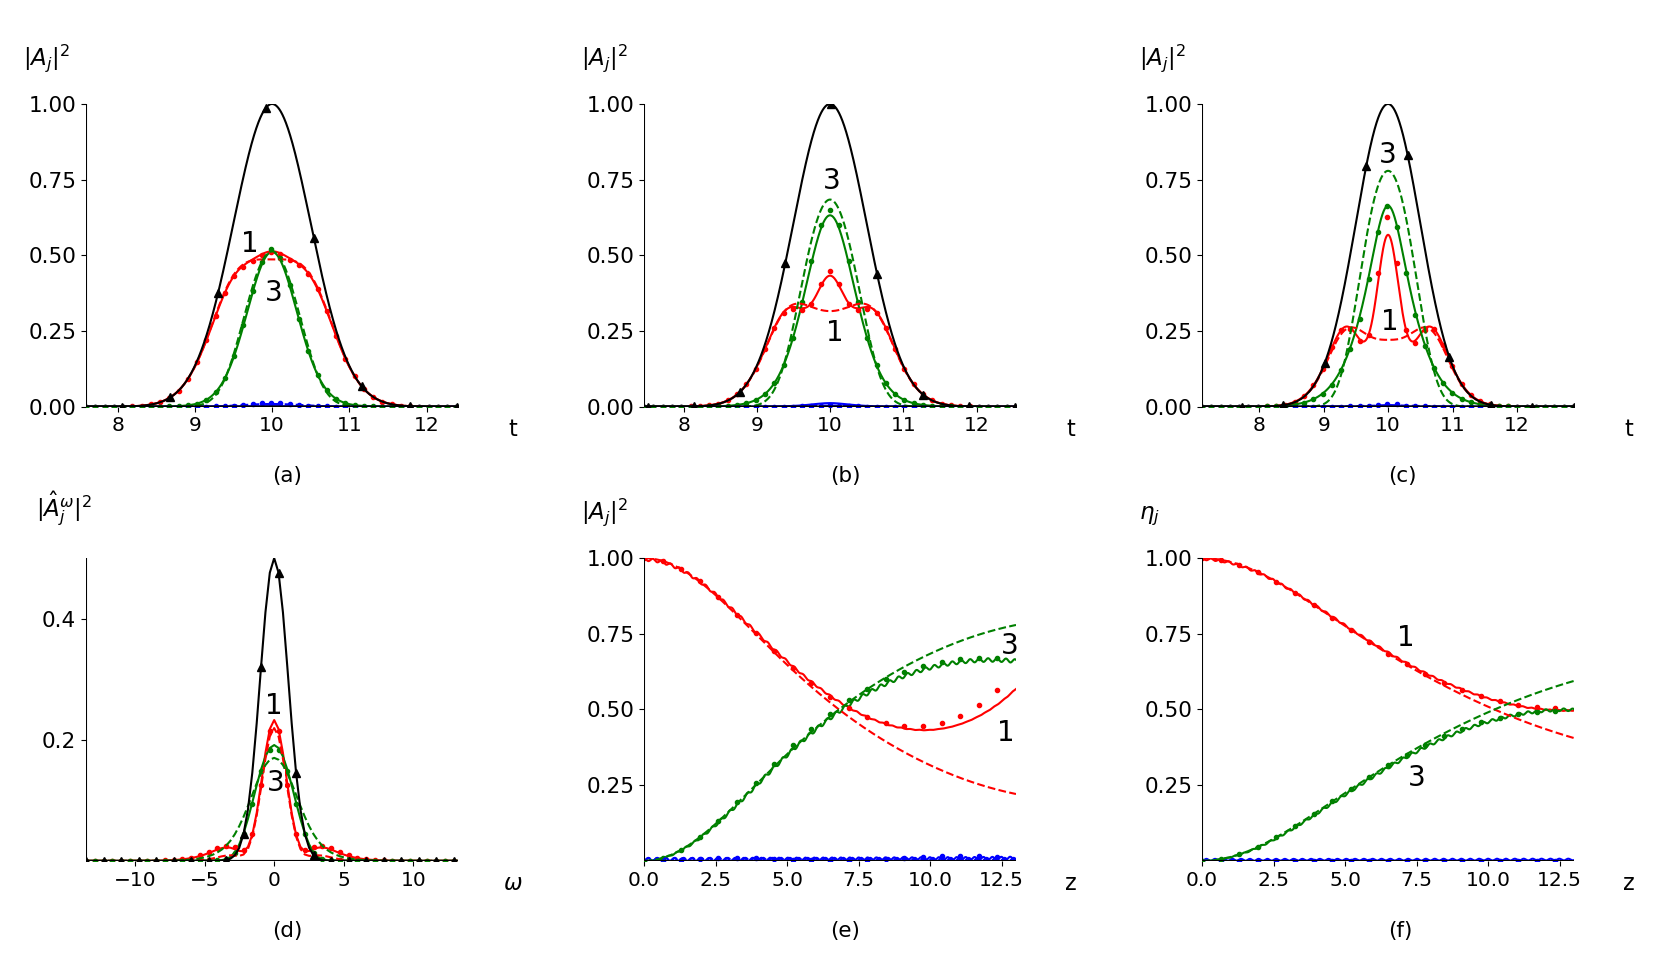
\includegraphics[width=\linewidth]{Cascade1_1}  
\caption{Pulse shapes in the sections \(z=7\) (a), \(10\) (b), \(13\) (c), and FW and TH spectra in the section \(z=13\) (d), and pulse intensities evolution at their centers (e) and the frequency conversion efficiency evolution (f) along \(z\)-coordinate computed for the parameters $\gamma=1,\, \Delta_{21} k=20,\, D_1=-0.0032,\, D_2=-0.0083,\, D_3=-0.0199.$ } 
\label{fr:c1_1}
\end{figure}

If the sign of the phase mismatching between FW and SH is negative (\(\Delta_{21}k=-20\)), then the energy conversion from the FW to TH also occurs with high efficiency (Fig.\ref{fr:c1_2}). Nevertheless, there are new essential features, which accompanies this process. 
\begin{figure}[h!] 
\centering 
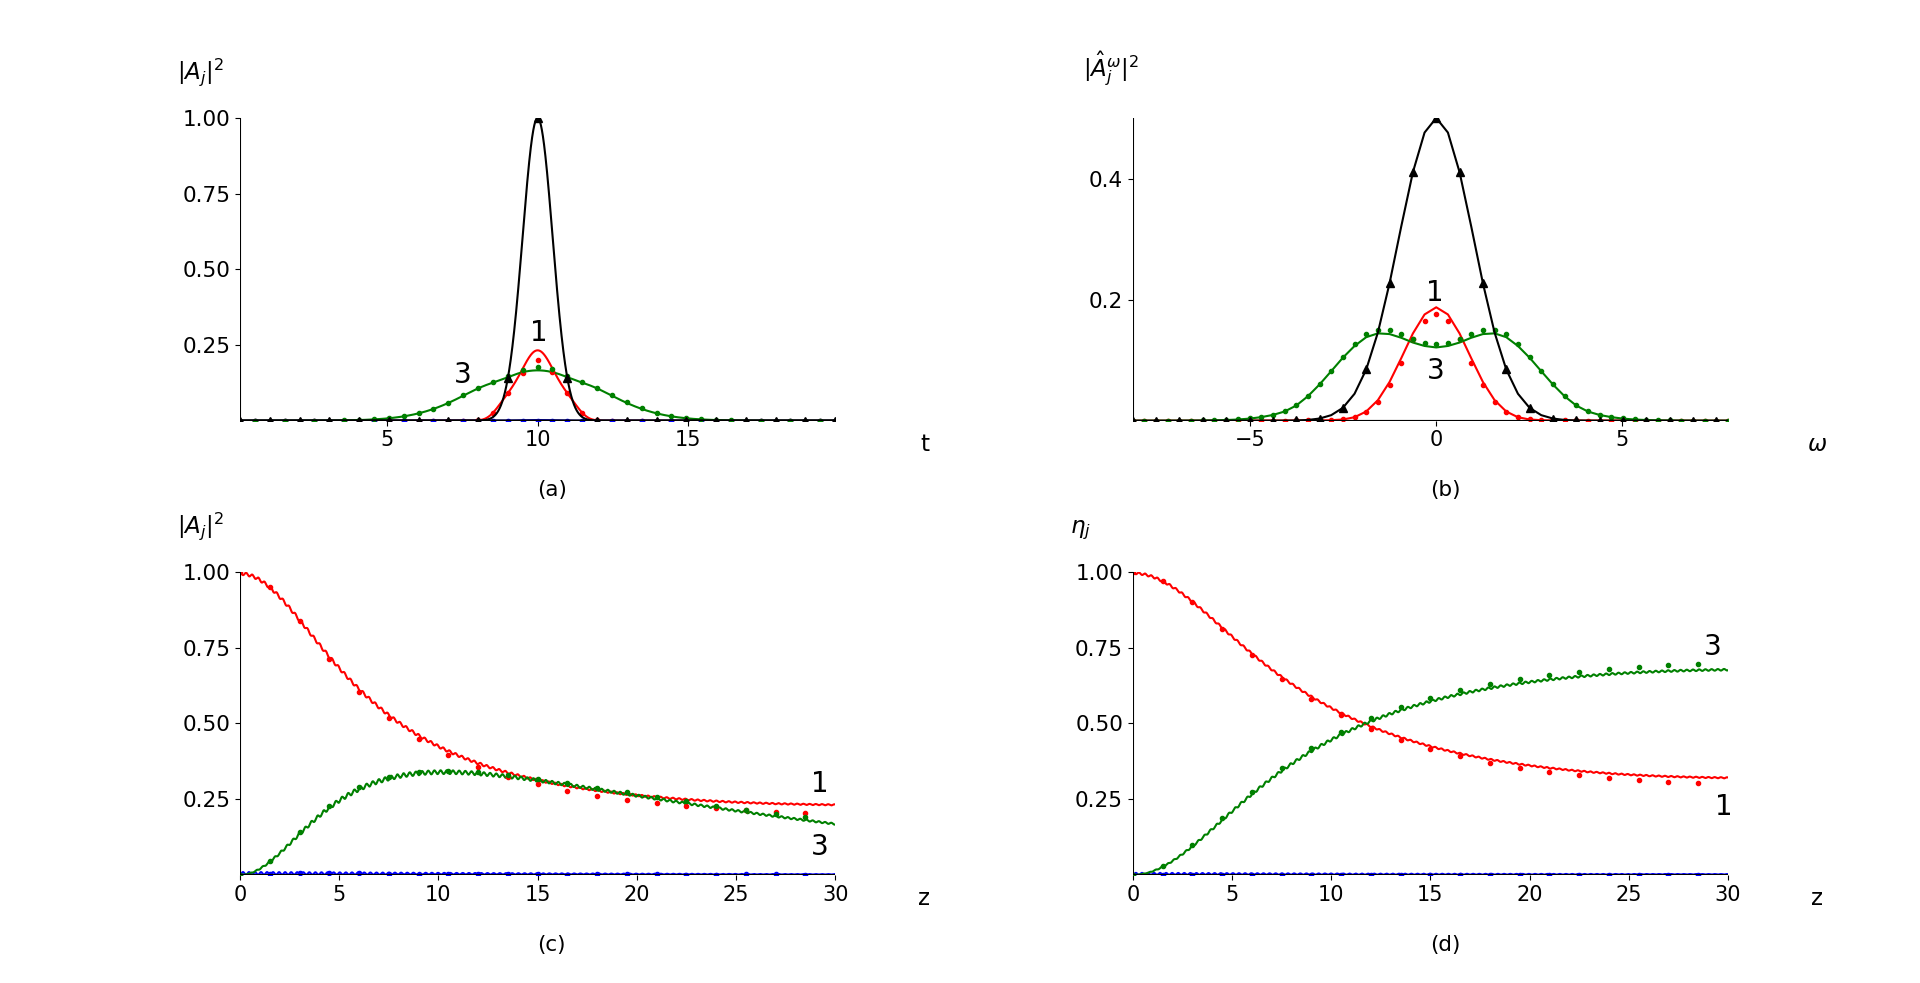
\includegraphics[width=0.9\linewidth]{Cascade1_2}  
\caption{Pulse shapes (a), FW and TH spectra (b) in the section \(z=30\), and pulse intensities evolution at their centers (c) and the frequency conversion efficiency evolution (d) along \(z\)-coordinate computed for the parameters $\gamma=1,\, \Delta_{21} k=-20,\, D_1=-0.0032,\, D_2=-0.0083,\, D_3=-0.0199.$} 
\label{fr:c1_2}
\end{figure}
So, this sign of the phase mismatching corresponds to FW pulse decompression due to induced cubic nonlinear response in a medium with normal dispersion. Therefore, the pulse duration of the FW and TH is greater than those at the positive phase mismatching (compare Fig. \ref{fr:c1_2} and Fig.\ref{fr:c1_1}). However, despite the FW pulse decompression, the bandwidth of the TH pulse spectrum is greater than the FW incident pulse spectrum. It means that the essential spectral broadening of the TH pulse occurs and this pulse can be additionally compressed. Moreover, the energy conversion reaches the value of about \(60\%\) at increased crystal length in comparison with the previous case: the crystal length must be about \(3\,cm\). Other features of the THG process are similar to the generation process at the positive phase mismatching.

\subsection{Anomalous dispersion of a medium at FW wavelength}
\label{par:an}
Let us briefly discuss THG in a medium with the anomalous dispersion occurring at the frequency of FW. Therefore, the SOD coefficient \(D_1\) is positive. We consider a propagation of the incident pulse with duration about \(100fs\) and with wavelength about \(1064nm\) in KDP crystal (see, for instance, \cite{bib:ri}). If \(\Delta_{21}k>0\) that corresponds to decompression of the FW pulse and compression of the pulse at trebled frequency, then the efficiency of FW energy conversion to the TH achieves about \(60\%\) in the section \(z=15\) (Fig. \ref{fr:c1_11}) and it is accompanied with TH pulse good shape and its broadened spectrum in comparison with the incident pulse spectrum at the FF. We see that the FW pulse shape has three intensity maxima and possesses smaller intensity at the pulse center in comparison with its value occurring at the pulse propagation in a medium possessing the normal dispersion at the FF. Nevertheless, we can see in Fig. \ref{fr:c1_11} that the FW pulse spectrum is more broadened in comparison with the incident pulse spectrum.

\begin{figure}[h!] 
\centering 
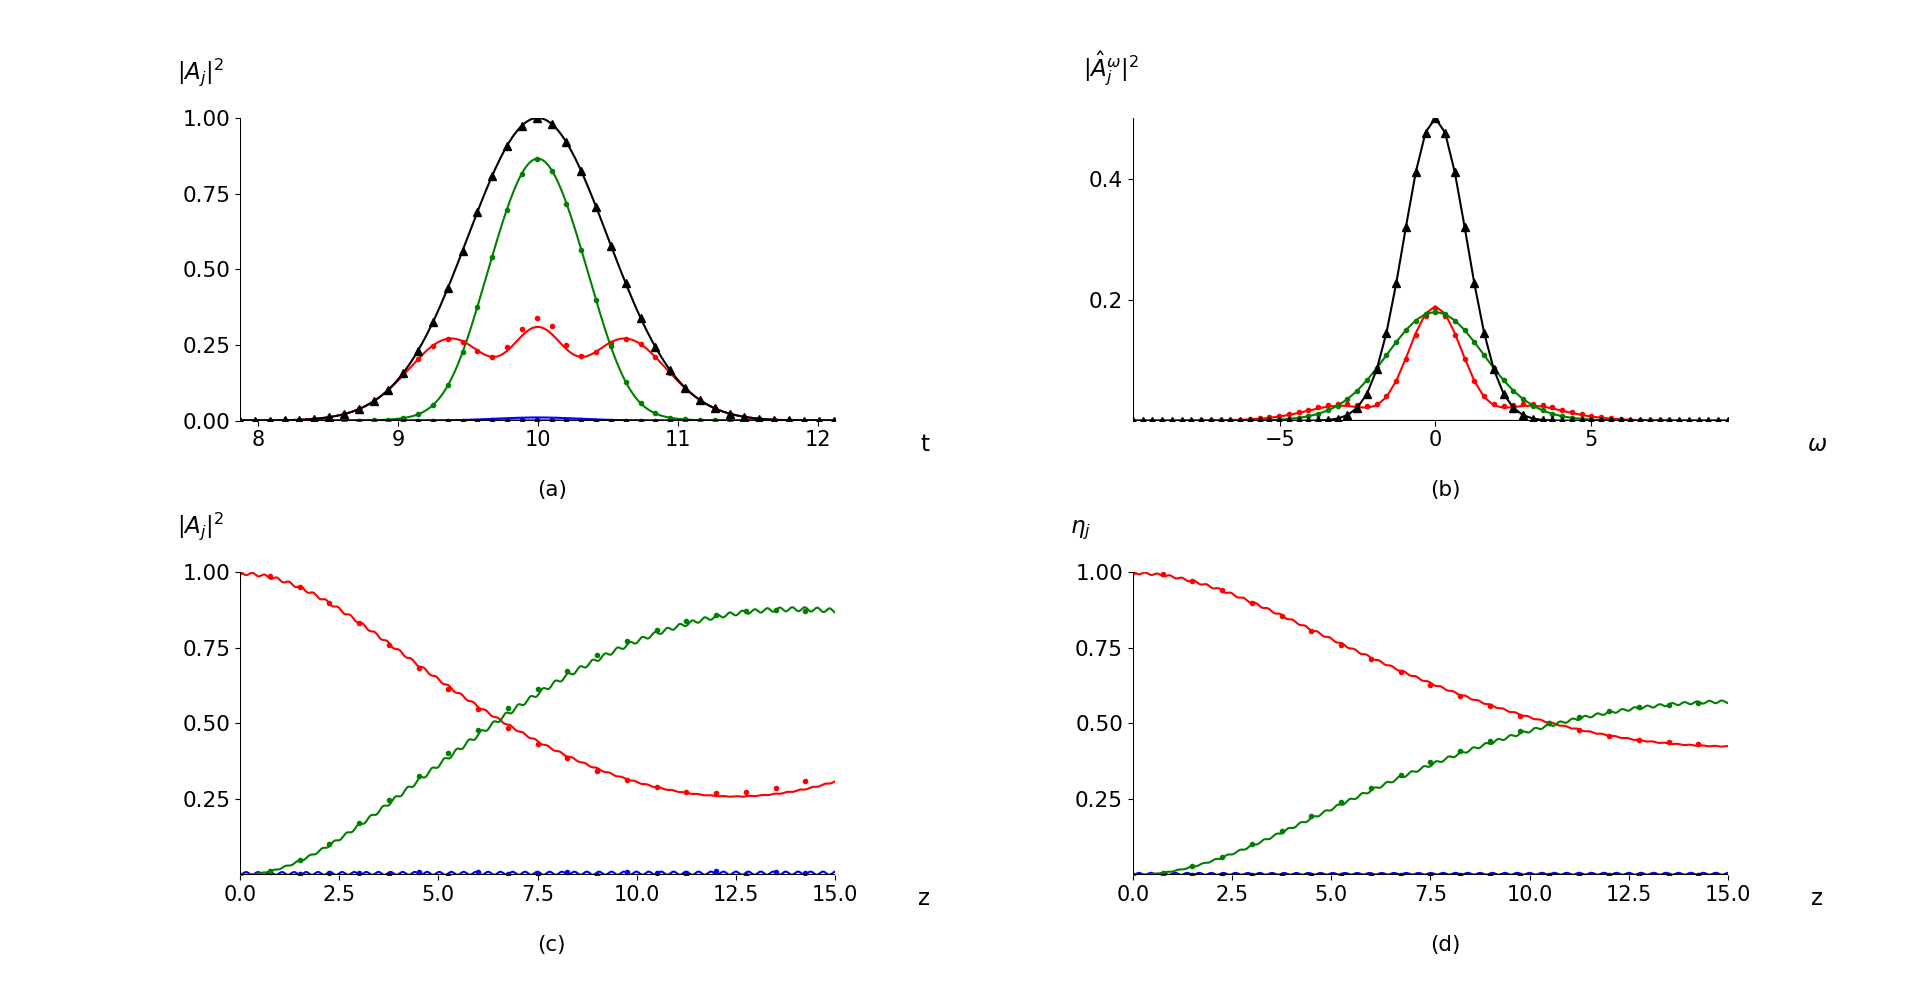
\includegraphics[width=0.9\linewidth]{Cascade1_11}  
\caption{Pulse shapes (a), and FW and TH spectra (b) in the section \(z=15\), and pulse intensities evolution at their center (c) and the frequency conversion efficiency evolution (d) along \(z\)-coordinate computed for the parameters  $\gamma=1,\, \Delta_{21} k=20,\, D_1=0.0006,\, D_2=-0.0035,\, D_3=-0.0062.$} 
\label{fr:c1_11}
\end{figure}

If the phase mismatching between FW and SH is negative (\(\Delta_{21}k<0\)), then the pulse compression at FF occurs, and decompression of the SH and TH pulses is observed. This leads to high-effective THG (Fig.\ref{fr:c1_12}): more than \(80\%\) of the FW energy converts to the TH wave! However, the TH intensity is less than its value at the positive phase mismatching \(\Delta_{21}k\), and the TH spectrum is smooth and broadened.

\begin{figure}[h!] 
\centering 
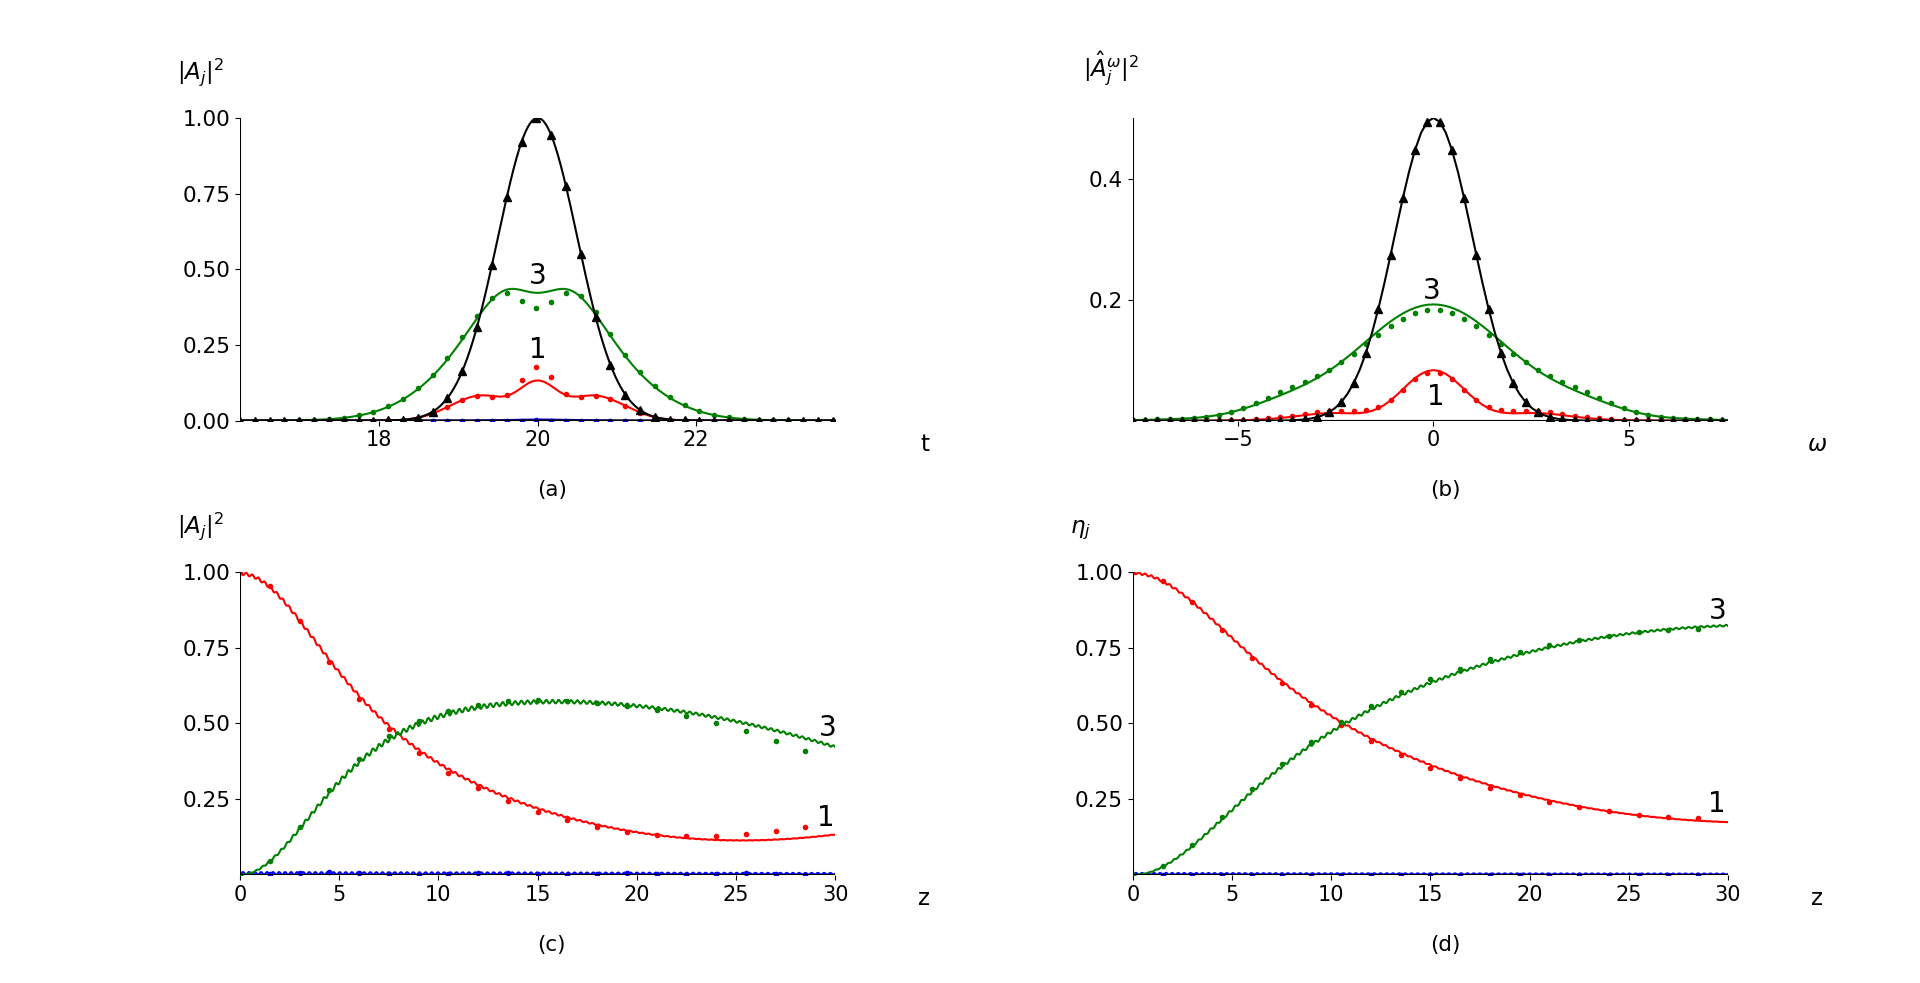
\includegraphics[width=0.9\linewidth]{Cascade1_12}  
\caption{Pulse shapes (a), and FW and TH spectra (b) in the section \(z=30\), and pulse intensities evolution at their center (c), and the frequency conversion efficiency evolution (d) along \(z\)-coordinate computed for the parameters  $\gamma=1,\, \Delta_{21} k=-20,\, D_1=0.0006,\, D_2=-0.0035,\, D_3=-0.0062.$} 
\label{fr:c1_12}
\end{figure}

\section{Conclusion and remarks}
We have proposed a new physical scheme of THG based on cascading SHG, which leads to an appearance of the induced cubic nonlinear response of a crystal possessing a quadratic susceptibility only. Thus, the frequency trebling is possible under the conditions corresponding to the frequency doubling of the laser pulse or beam. The generation process is not restricted by the incident pulse duration. A necessary length of a crystal, at which an efficient THG is observed, depends on the phase mismatching between the SH and FW and can be changed from 1.0 cm to 20 cm. 

Using multiscale method, we have derived the equations (named as modified equations) describing frequency trebling due to cascading SHG and showed that they contain the terms responsible for the cubic nonlinear response, which results in THG as well as FW self-modulation, and also FW and TH cross-modulation. Essentially, the equations do not contain the term responsible for the TH self-modulation that is very important for practice.A validity of the modified equations is confirmed by comparing of solutions of both sets of the Schr\"{o}dinger equations: original ones and modified ones. We developed an analytical solution of the modified equations in the framework of the long pulse duration approximation at using the derived integrals of motion. This solution allows us to estimate a maximal frequency conversion efficiency as well as its dependence on the parameters of interacting waves.

In Supplementary Information we provide another computer simulation results of frequency tripling. Highly intensive THG is achieved for both positive and negative phase mismatching between SH and FW. At the negative sign of the phase mismatching, the MI may appear, and as a result of this, a dramatic decreasing of the THG efficiency occurs. Nevertheless, at the beginning stage of the MI, a regular sequence of very short sub-pulses with self-similar shapes may appear.

We have also investigated the influence of other parameters on the pulse interaction: SOD, and the phase mismatching between TH and FW, and GVM between both SH and FW as well as TH and FW.  We show that the high THG efficiency is achieved for both types of a medium: anomalous and normal dispersion at the FF. The GVM between SH and FW pulses influences only the pulse shapes without strong changing of the THG efficiency. In contrast, the GVM between TH and FW influences remarkably the frequency conversion process. To compensate this negative influence, we have proposed and discussed some physical schemes for three-waves interaction. Moreover, since only quadratic nonlinear effects are required for THG through the cascading SHG, it is possible to use longer pulses with duration of picoseconds or nanoseconds to decrease negative GVM and SOD influence. Another way is using of so-called "tilted pulses" \cite{bib:tilt1,bib:tilt2} to compensate SOD effects.
%\clearpage
\begin{thebibliography}{0}
\bibitem{bib:n1} Karamzin, Yu.N., Sukhorukov, A.P. Nonlinear interaction of diffracted light beams in a medium with quadratic nonlinearity: mutual focusing of beams and limitation on the efficiency of optical frequency converters. \textit{JETP Lett.} \textbf{20}, 339 (1974).
\bibitem{bib:n2} Torruellas, W.E. et al. Observation of two-dimensional spatial solitary waves in a quadratic medium. \textit{Physical review letters} \textbf{74}, 5036 (1995).
\bibitem{bib:n3} Schiek, R., Baek, Y., Stegeman, G. I. One-dimensional spatial solitary waves due to cascaded second-order nonlinearities in planar waveguides. \textit{Physical Review E} \textbf{53}, 1138 (1996).
\bibitem{bib:n4} Fuerst, R. A. et al. Spatial modulational instability and multisolitonlike generation in a quadratically nonlinear optical medium. \textit{Physical review letters} \textbf{78}, 2756 (1997).
\bibitem{bib:n5} Costantini, B. et al. Collisions between type II two-dimensional quadratic solitons. \textit{Optics letters} \textbf{23}, 424-426 (1998).
\bibitem{bib:n6} Di Trapani, P. et al. Observation of temporal solitons in second-harmonic generation with tilted pulses. \textit{Physical review letters} \textbf{81},570 (1998).
\bibitem{bib:n7} Liu, X., Qian, L. J., Wise, F. W. Generation of optical spatiotemporal solitons. \textit{Physical review letters} \textbf{82}, 23 (1999).
\bibitem{bib:n9} Kim, D. H., Kang, J. U., Khurgin, J. B. Cascaded Raman self-frequency shifted soliton generation in an Er/Yb-doped fiber amplifier. \textit{Applied physics letters} \textbf{81}, 2695 (2002).
\bibitem{bib:n10} Kharenko, D. S. et al. Cascaded generation of coherent Raman dissipative solitons \textit{Optics letters} \textbf{41}, 175 (2016).
\bibitem{bib:n8} Buryak, A. V. et al. Optical solitons due to quadratic nonlinearities: from basic physics to futuristic applications. \textit{Physics Reports} \textbf{370}, 63 (2002).
\bibitem{bib:n11} Cheng, Z., Fu, H. Y., Li, Q. Cascaded photonic crystal fibers for three stage non-integer order soliton compression. \textit{Optical Communications and Networks}, 1 (2017).
\bibitem{bib:n12} Bache, M., Wise, F. W. Type-I cascaded quadratic soliton compression in lithium niobate: Compressing femtosecond pulses from high-power fiber lasers. \textit{Physical Review A} \textbf{81}, 053815 (2010).
\bibitem{bib:n13} Zeng, X. et al. Adiabatic femtosecond pulse compression and control by using quadratic cascading nonlinearity \textit{Nonlinear Optics: Technologies and Applications. -- International Society for Optics and Photonics} \textbf{6839}, 68390B (2008).
\bibitem{bib:n14} Ashihara, S. et al. Soliton compression of femtosecond pulses in quadratic media. \textit{JOSA B} \textbf{19}, 2505 (2002).
\bibitem{bib:n15} Li, Q., Kutz, J. N., Wai, P. K. A. Cascaded higher-order soliton for non-adiabatic pulse compression. \textit{JOSA B} \textbf{27}, 2180 (2010).
\bibitem{bib:n16} Bache, M. et al. Limits to compression with cascaded quadratic soliton compressors. \textit{Optics express} \textbf{16}, 3273 (2008).
\bibitem{bib:n17} Moses, J., Wise, F. W. Soliton compression in quadratic media: high-energy few-cycle pulses with a frequency-doubling crystal. \textit{Optics letters} \textbf{31}, 1881 (2006).
\bibitem{bib:n18} \v{S}uminas. R. et al. Spatiotemporal light bullets and supercontinuum generation in $\beta$-BBO crystal with competing quadratic and cubic nonlinearities \textit{Optics letters} \textbf{41}, 2097 (2016).
\bibitem{bib:n19} Conti, C., et al. Effective lensing effects in parametric frequency conversion. \textit{JOSA B} \textbf{19},  852 (2002).
\bibitem{bib:n20} Trofimov, V. A., Lysak T. M. Strong self-focusing of axial symmetric laser beam due to quadratic nonlinearity. \textit{JOSA B} \textbf{29}, 1731 (2012).
\bibitem{bib:n21} Lysak, T. M., Trofimov, V. A. Achieving high-efficiency second harmonic generation in a sequence of laser pulses with random peak intensity. Part I. Efficient generation in optical fibers. \textit{Computational Mathematics and Modeling} \textbf{19}, 333 (2008).
\bibitem{bib:n22} Lysak, T. M., Trofimov, V. A. Achieving high-efficiency second harmonic generation in a sequence of laser pulses with random peak intensity. Part II. Suppression of intensity fluctuations in a quadratic-nonlinearity medium \textit{Computational Mathematics and Modeling} \textbf{20}, 1 (2009).
\bibitem{bib:n23a} Lysak, T. M., Trofimov, V. A. Achieving high-efficiency second harmonic generation in a sequence of laser pulses with random peak intensity. Part III. Propagation of pulses in a bulk medium. \textit{Computational Mathematics and Modeling} \textbf{20}, 101 (2009).
\bibitem{bib:n23} Lysak, T. M., Trofimov, V. A. Highly efficient SHG of a sequence of laser pulses with a random peak intensity and duration. \textit{Optics and Spectroscopy} \textbf{107}, 399 (2009).
\bibitem{bib:n24} Nayfeh, A.H. Introduction to perturbation techniques.\textit{New York: John Wiley \&Sons} (1993) 519p.
\bibitem{bib:t4} Craxton, R. S. Theory of high efficiency third harmonic generation of high power Nd-glass laser radiation. \textit{Optics Communications} \textbf{34}, 474 (1980).

\bibitem{bib:t3} Qi, H. et al. Cascaded third-harmonic generation with one KDP crystal. \textit{Optics letters} \textbf{41} 5823 (2016).
\bibitem{bib:t1} Banks, P. S., Feit, M. D., Perry, M. D. High-intensity third-harmonic generation. \textit{JOSA B} \textbf{19}, 102 (2002).
\bibitem{bib:t2} Zhu, S. N., Zhu, Y. Y., Ming, N. B. Quasi-phase-matched third-harmonic generation in a quasi-periodic optical superlattice. \textit{Science} \textbf{278}, 843 (1997)
\bibitem{bib:t5} Zhang, Tiejun, Yoshiaki Kato, and Hiroyuki Daido. "Efficient third-harmonic generation of a picosecond laser pulse with time delay." IEEE journal of quantum electronics 32.1 (1996): 127-136.
\bibitem{bib:ri} https://refractiveindex.info
\bibitem{bib:tilt1} Martinez, O. E., Gordon, J. P., Fork, R. L. Negative group-velocity dispersion using refraction \textit{JOSA A}, \textbf{1} 1003 (1984).
\bibitem{bib:tilt2} Martinez, O. E. Grating and prism compressors in the case of finite beam size. \textit{JOSA B} \text{3}, 929 (1986).
\end{thebibliography}
\section*{Methods}
\subsection*{Invariants of the modified equations}
To derive the energy invariant, we multiply the equations \eqref{eq:main2} on \(U^*\) and \(W^*\), respectively, and multiply the ones, conjugated to them, on \(U\) and \(W\):
\[
\begin{aligned}
&\frac{\partial U}{\partial z}U^*+iD_1\frac{\partial^2 U}{\partial t^2}U^*-i\frac{\gamma^2}{\Delta_{21} k}(|U|^4+3U^{*3}W+2|U|^2|W|^2)=0,\\
&\frac{\partial U^*}{\partial z}U-iD_1\frac{\partial^2 U^*}{\partial t^2}U+i\frac{\gamma^2}{\Delta_{21} k}(|U|^4+3U^{3}W^*+2|U|^2|W|^2)=0,\\
&\frac{\partial W}{\partial z}W^*+\nu_{31}\frac{\partial{W}}{\partial t}W^*+iD_3\frac{\partial^2 W}{\partial t^2}W^*-3i\frac{\gamma^2}{\Delta_{21} k}(U^3W^*+2|U|^2|W|^2)+i\Delta_{31}k|W|^2=0.\\
&\frac{\partial W^*}{\partial z}W+\nu_{31}\frac{\partial{W^*}}{\partial t}W+iD_3\frac{\partial^2 W^*}{\partial t^2}W+3i\frac{\gamma^2}{\Delta_{21} k}(U^{*3}W+2|U|^2|W|^2)-i\Delta_{31}k|W|^2=0.\\
\end{aligned}
\]
Then we take a sum of these equations and integrate this sum with respect to time from \(0\) to \(L_t\):
\[
\begin{aligned}
&\frac{d}{dz}\int\limits_0^{L_t}\left(|U|^2+|W|^2\right)dt+\nu_{31}\int\limits_0^{L_t}\left(\frac{\partial{W}}{\partial t}W^*+\frac{\partial{W^*}}{\partial t}W\right)dt\\
&+i\int\limits_0^{L_t}\left(D_1(\frac{\partial^2 U}{\partial t^2}U^*-\frac{\partial^2 U^*}{\partial t^2}U)+D_3(\frac{\partial^2 W}{\partial t^2}W^*-\frac{\partial^2 W^*}{\partial t^2}W)\right)dt=0.
\end{aligned}
\]
Since \(U,\,W\) are equal to zero at the time moments \(t=0\) and \(t=L_t\), then the second integral equals zero. Integrating by parts in the last integral and taking into account the BCs, one can see that the third integral also equals zero.  Hence, the equation set \eqref{eq:main2} possesses the energy conservation law (the first invariant): 

\begin{equation}
\label{eq:ninv1}
I_1=\int\limits_0^{L_t}\left(|U|^2+|W|^2\right)dt=const
\end{equation}

To derive the Hamiltonian of the equation set (the third invariant), we have to state additional conditions for the complex amplitudes: their first time derivatives must be equal to zero at the time moments \(t=0\) and \(t=L_t\):
\[\frac{\partial U}{\partial t}|_{t=0}=\frac{\partial U}{\partial t}|_{t=L_t}=\frac{\partial W}{\partial t}|_{t=0}=\frac{\partial W}{\partial t}|_{t=L_t}=0\]
or values of these derivatives tend to zero if time tends to infinity for the unbounded time domain. However, since we consider the finite distributions for the incident pulse, then the additional conditions do not restrict our analysis.

To derive the Hamiltonian, we multiply the equations \eqref{eq:main2} on \(\frac{\partial U^*}{\partial z},\,\frac{\partial W^*}{\partial z}\), respectively, and multiply the equations, conjugated to them, on \(\frac{\partial U}{\partial z},\,\frac{\partial W}{\partial z}\), respectively:
\[
\begin{aligned}
&\frac{\partial U}{\partial z}\frac{\partial U^*}{\partial z}+iD_1\frac{\partial^2 U}{\partial t^2}\frac{\partial U^*}{\partial z}-i\frac{\gamma^2}{\Delta_{21} k}((|U|^2+2|W|^2)U\frac{\partial U^*}{\partial z}+3U^{*2}\frac{\partial U^*}{\partial z}W)=0,\\
&\frac{\partial U}{\partial z}\frac{\partial U^*}{\partial z}-iD_1\frac{\partial^2 U^*}{\partial t^2}\frac{\partial U}{\partial z}+i\frac{\gamma^2}{\Delta_{21} k}((|U|^2+2|W|^2)U^*\frac{\partial U}{\partial z}+3U^{2}\frac{\partial U}{\partial z}W^*)=0,\\
&\frac{\partial W}{\partial z}\frac{\partial W^*}{\partial z}+\nu_{31}\frac{\partial W}{\partial t}\frac{\partial W^*}{\partial z}+iD_3\frac{\partial^2 W}{\partial t^2}\frac{\partial W^*}{\partial z}-3i\frac{\gamma^2}{\Delta_{21} k}(U^3\frac{\partial W^*}{\partial z}+2|U|^2\frac{\partial W^*}{\partial z}W)+i\Delta_{31}kW\frac{\partial W^*}{\partial z}=0.\\
&\frac{\partial W}{\partial z}\frac{\partial W^*}{\partial z}+\nu_{31}\frac{\partial W^*}{\partial t}\frac{\partial W}{\partial z}-iD_3\frac{\partial^2 W^*}{\partial t^2}\frac{\partial W}{\partial z}+3i\frac{\gamma^2}{\Delta_{21} k}(U^{*3}\frac{\partial W}{\partial z}+2|U|^2\frac{\partial W}{\partial z}W^*)-i\Delta_{31}kW^*\frac{\partial W}{\partial z}=0.\\
\end{aligned}
\]
Then, we subtract from the equations the corresponding conjugated ones, so we obtain
\begin{footnotesize}
\[
\begin{aligned}
&D_1\left(\frac{\partial^2 U}{\partial t^2}\frac{\partial U^*}{\partial z}+\frac{\partial^2 U^*}{\partial t^2}\frac{\partial U}{\partial z}\right)-\frac{\gamma^2}{\Delta_{21}k}\left((|U|^2+2|W|^2)\frac{\partial|U|^2}{\partial z}+\frac{\partial U^{*3}}{\partial z}W+\frac{\partial U^{3}}{\partial z}W^*\right)=0,\\
&\nu_{31}\left(\frac{\partial W}{\partial t}\frac{\partial W^*}{\partial z}-\frac{\partial W^*}{\partial t}\frac{\partial W}{\partial z}\right)+D_3\left(\frac{\partial^2 W}{\partial t^2}\frac{\partial W^*}{\partial z}+\frac{\partial^2 W^*}{\partial t^2}\frac{\partial W}{\partial z}\right)-\frac{3\gamma^2}{\Delta_{21}k}\left(2|U|^2\frac{\partial |W|^2}{\partial z}-U^3\frac{\partial W^*}{\partial z}-U^{*3}\frac{\partial W}{\partial z}\right)+\Delta_{31}k\frac{\partial|W|^2}{\partial z}=0.\\
\end{aligned}
\]
\end{footnotesize}
After that, we multiply the first equation on \(6\) and the second equation on \(2\) and take a sum:
\[
\begin{aligned}
\int\limits_0^{L_t}\Big(&2\nu_{31}\left(\frac{\partial W}{\partial t}\frac{\partial W^*}{\partial z}-\frac{\partial W^*}{\partial t}\frac{\partial W}{\partial z}\right)+6D_1\left(\frac{\partial^2 U}{\partial t^2}\frac{\partial U^*}{\partial z}+\frac{\partial^2 U^*}{\partial t^2}\frac{\partial U}{\partial z}\right)+2D_3\left(\frac{\partial^2 W}{\partial t^2}\frac{\partial W^*}{\partial z}+\frac{\partial^2 W^*}{\partial t^2}\frac{\partial W}{\partial z}\right)\\
+&\frac{\gamma^2}{\Delta_{21}k}\frac{\partial}{\partial z}\left(-12Re(U^3W^*)-3|U|^4-12|U|^2|W|^2\right)+2\Delta_{31}k\frac{\partial |W|^2}{\partial z}\Big)dt=0.
\end{aligned}
\]
Using the integration by parts, we show that the equation set \eqref{eq:main2} possesses the Hamiltonian (the third invariant):

\begin{equation}
\label{eq:ninv3}
\begin{aligned}
I_3&=\int\limits_0^{L_t}\Big(2\nu_{31}Im\left(W^*\frac{\partial W}{\partial t}\right)-6D_1|\frac{\partial U}{\partial t}|^2-2D_3|\frac{\partial W}{\partial t}|^2-\\
&\frac{3\gamma^2}{\Delta_{21}k}\left(4Re(U^3W^*)+|U|^4+4|U|^2|W|^2\right)+2\Delta_{31}k|W|^2\Big)dt=const.
\end{aligned}
\end{equation}

For clarity, it should be stressed that the original set of equations also possesses some invariants:
\begin{equation}
\label{eq:inv1}
\begin{aligned}
&I_1=\int\limits_0^{L_t}\left(|A_1|^2+|A_2|^2+|A_3|^2\right)dt\\
\end{aligned}
\end{equation}
--the first invariant (the energy preservation law),
\begin{equation}
I_2=\int\limits_0^{L_t}\left(\sum\limits_{j=1}^3 p_j A_j \frac{\partial A_j^*}{\partial t}\right)dt,\,p_1=6,\, p_2=3,\, p_3=2
\end{equation}
--the second invariant (the impulse preservation law),
\begin{equation}
\label{eq:inv3}
\begin{aligned}
&I_3=\int\limits_0^{L_t}\Big(-\sum\limits_{j=1}^3 p_jD_j |\frac{\partial A_j}{\partial t}|^2-\nu_{21}Im\left(A_2^*\frac{\partial A_2}{\partial t}\right)-\nu_{31}Im\left(A_3^*\frac{\partial A_3}{\partial t}\right)+6\gamma Re\bigl(2A_1 A_2 A_3^*e^{i(\Delta_{31}k-\Delta_{21}k)z}\\
&+A_1^2 A_2^*e^{\Delta_{21}k\cdot z}\bigr)+\alpha\big(4Re\bigl({A_1^3}{A_3^*}e^{i\Delta_{31}k\cdot z}+3{A_1^*}{A_2^2}{A_3^*}e^{-i(2\Delta_{21}k-\Delta_{31}k)z}\bigr)+3({|A_1|^4}+{|A_2|^4}+{|A_3|^4})\\
&+12({|A_1|^2}{|A_2|^2}+{|A_1|^2}{|A_3|^2}+{|A_2|^2}{|A_3|^2}))+3\Delta_{21} k|A_2|^2+2\Delta_{31} k|A_3|^2\Big)dt,\,p_1=6,\, p_2=3,\, p_3=2
\end{aligned}
\end{equation}
-- the third invariant (Hamiltonian). Let us notice that for unbounded time domain the integration limits change on \(\{-\infty,\infty\}\), respectively. 

We want to emphasize that the value of the first invariant \eqref{eq:ninv1} and the value of the first invariant \eqref{eq:inv1} for the original set of the equations coincide with each other and they are equal to \(\int\limits_0^{L_t}|A_{10}|^2dt\). However, because the invariant for the modified set of equations does not contain the SH wave, then the sum energy of two waves will be greater than a sum of the energies of corresponding waves defined as the solution of the original problem.

\subsection*{Exact solution of the modified problem.}
In the framework of the long pulse duration approximation, the functions \(U,W\) depend only on \(z\) coordinate, and we can rewrite the problem \eqref{eq:main2},\eqref{eq:ini2} in the form
\begin{equation}
\label{eq:main2l}
\begin{aligned}
&\frac{dU}{dz}-i\frac{\gamma^2}{\Delta_{21} k}(|U|^2U+3U^{*2}W+2U|W|^2)=0,\\
&\frac{dW}{dz}-3i\frac{\gamma^2}{\Delta_{21} k}(U^3+2|U|^2W)+\Delta_{31}kW=0,\,  0< z \leq L_z\\
&U(0)=1,\,W(0)=0.\\
\end{aligned}
\end{equation}

The invariants \eqref{eq:ninv1}, \eqref{eq:ninv3} are written as
\begin{equation}
\label{eq:ninvs}
\begin{aligned}
&I_1=|U|^2+|W|^2,\\
&I_3=\frac{\gamma^2}{\Delta_{21}k}\left(-12Re(U^3W^*)-3|U|^4-12|U|^2|W|^2\right)+2\Delta_{31}k|W|^2.
\end{aligned}
\end{equation}
We note that the first invariant of the problem \eqref{eq:main2l} equals unity (\(I_1=1\)) due to the initial conditions.

To obtain the interacting waves intensities evolution, we use a well-known representation for the complex amplitudes:
\begin{equation}
\label{eq:repr}
U(z)=a_1e^{i\varphi_1(z)},\,W(z)=a_3e^{i\varphi_3(z)},
\end{equation}
where \(a_j,\,\varphi_j\) are real functions and \(\varphi_1,\,\varphi_3\) describe the phase evolution of waves and \(a_1^2;\, a_3^2\) are the wave intensities. In new notations the equations \eqref{eq:main2l} takes the form:
\begin{equation}
\label{eq:main3}
\begin{aligned}
&\frac{da_1}{dz}=-\frac{3\gamma^2}{\Delta_{21}k}a_1^2a_3\sin\varphi,\\
&\frac{da_3}{dz}=\frac{3\gamma^2}{\Delta_{21}k}a_1^3\sin\varphi,\\
&\frac{d\varphi}{dz}-\frac{\gamma^2}{\Delta_{21}k}\left(3\left(\frac{a_1^3}{a_3}-3a_1a_3\right)\cos\varphi+3a_1^2-6a_3^2\right)+\Delta_{31}k=0,
\end{aligned}
\end{equation}
here \(\varphi=\varphi_3-3\varphi_1\) is a phase difference between TH and FW. The invariants \eqref{eq:ninvs} are written as
\[
\begin{aligned}
&I_1=a_1^2+a_3^2=1,\\
&I_3=\frac{\gamma^2}{\Delta_{21}k}\left(-12a_1^3a_3\cos\varphi-3a_1^4-12a_1^2a_3^2\right)+\Delta_{31}ka_3^2.
\end{aligned}
\]
We modify the third invariant to express \(\cos \varphi\):
\[
\tilde{I}_3=I_3+3\frac{\gamma^2}{\Delta_{21}k}I_1^2=-12\frac{\gamma^2}{\Delta_{21}k}a_1^3a_3\cos\varphi+-6\frac{\gamma^2}{\Delta_{21}k}a_1^2a_3^2+3\frac{\gamma^2}{\Delta_{21}k}a_3^4+2\Delta_{31}ka_3^2=0,
\]
which equals zero because the TH incident intensity is equal to zero: \(a_3(0)=0\). Hence, we can express \(\cos \varphi\):
\begin{equation}
\label{eq:cos}
\cos\varphi=\frac{a_3(-6a_1^2+3a_3^2+2p)}{12a_1^3},
\end{equation}
\textcolor{ForestGreen}{where parameter $p$ is defined in the main part of the paper}. Obviously,  inequality 
\[
|\cos\varphi|\le1
\]
 must be valid. Then we find \(\sin \varphi\) from the equality \eqref{eq:cos} and substitute it into the first equation of the equation set \eqref{eq:main3}, which is preliminary multiplied by \(a_1\). As a result, we write the following equation with respect to the TH intensity:
\[\frac{da_1^2}{dz}=\mp6\frac{\gamma^2}{\Delta_{21}k}a_1^3a_3(\sqrt{1-\frac{a_3^2(-6a_1^2+3a_3^2+2p)^2}{36a_1^6}}.\]
Using the new variable \(p_1=a_1^2\) and expressing \(a_1^2\) from the first invariant \(a_3^2=1-p_1\), we finally obtain:
\begin{equation}
\label{eq:main4}
\begin{aligned}
&\frac{dp_1}{dz}=\mp7.5\frac{\gamma^2}{\Delta_{21}k}\sqrt{(1-p_1)f(p_1)},\\
&f(p_1)=\frac{16}{25}(p_1^3-\frac{1}{144}(1-p_1)(-9p_1+2p+3)^2).
\end{aligned}
\end{equation}
Sign in the right side of the equation corresponds to different processes: sign ``minus" corresponds to THG and sign ``plus" to reverse energy transfer from the wave with trebled frequency to the FW. So, since TH incident intensity equals zero, then we choose the sign ``minus".

\textcolor{ForestGreen}
{
Obviously, the solution depends on the parameter $p$. In fact, there are different areas of waves interaction. These areas are defined by the number of real roots of the equation
$$
f(p_1)=0,
$$
which can be found by using the Sturm theorem. We will further the notation $P_{11},\,P_{12},\,P_{13}$ for the roots of this equation, where $P_{11}$ is always real, and, if two other roots are also real, then $P_{11}\ge P_{12}\ge P_{13}$. It should be also stressed that the equation \eqref{eq:main4} can be resolved, generally through elliptical function, or through elementary functions. Below, we briefly present the main results.
\paragraph*{Case $p<-1.5,\,p>3 + \frac{9}{\sqrt[3]{2}}-9\sqrt[3]{ 2}$: two complex roots $P_{12},P_{13}$.}
In this case only root $P_{11}$ is positive, so $p_1(z)$ changes between $1$ and $P_{11}$ by the following formula:
\begin{equation}
\label{eq:p1_1}
p_1(z)=\frac{(d-cP_{11})cn(7.5\frac{\gamma^2}{\Delta_{21}k}\kappa z,k)+(cP_{11}+d)}{(d-c)cn(7.5\frac{\gamma^2}{\Delta_{21}k}\kappa z,k)+(c+d)},
\end{equation}
where
$$
\begin{aligned}
&c=\sqrt{(1-r)^2+s^2},\, d=\sqrt{(p_{11}-r)^2+s^2}, \kappa=\sqrt{cd}, k=\frac{\kappa^2+(r-P_{11})(1-r)-s^2}{2\kappa^2},\\
&r=Re(P_{12}),\, s=Im (P_{12}).
\end{aligned}
$$
\paragraph*{Case: $-1.5<p<3 + \frac{9}{\sqrt[3]{2}}-9\sqrt[3]{ 2}$: three real roots}
Under such condition, all three roots $P_{1j}$ are positive, so there are two regimes of waves interaction: low-effective and high-effective. In low-effective regime, the FW intensity changes between $1$ and $P_{11}$ by the formula
\begin{equation}
\label{eq:p1_2}
\begin{aligned}
&p_1(z)=\frac{(1-P_{11})P_{13}sn^2(7.5\frac{\gamma^2}{\Delta_{21}k}\sqrt{(1-P_{12})(P_{11}-P_{13})}z,k)+(P_{11}-P_{13})}{(1-P_{11})sn^2(7.5\frac{\gamma^2}{\Delta_{21}k} \sqrt{(1-P_{12})(P_{11}-P_{13})}z,k)+(P_{11}-P_{13})},\\
&k=\sqrt{\frac{(1-P_{11})(P_{12}-P_{13})}{(1-P_{12})(P_{11}-P_{13})}}.
\end{aligned}
\end{equation} 
In high-effective regime, the FW intensity changes between $P_{12}$ and $P_{13}$ by the formula
\begin{equation}
\label{eq:p1_2bis}
\begin{aligned}
&p_1(z)=\frac{(P_{12}-P_{13})sn^2(7.5\frac{\gamma^2}{\Delta_{21}k}\sqrt{(1-P_{12})(P_{11}-P_{13})}z,k)+(1-P_{12})P_{13}}{(P_{12}-P_{13})sn^2(7.5\frac{\gamma^2}{\Delta_{21}k}\sqrt{(1-P_{12})(P_{11}-P_{13})}z,k)+(1-P_{12})},\\
&k=\sqrt{\frac{(1-P_{11})(P_{12}-P_{13})}{(1-P_{12})(P_{11}-P_{13})}}.
\end{aligned}
\end{equation}
\paragraph*{Special case $p=-1.5$: $0=P_{13}=P_{12}<P_{11}<1$}
So, here $p_1(z)$ once again changes between $1$ and $P_{11}=0.36$, but now, it is expressed through cosine function:
\begin{equation}
\label{eq:p1_3}
p_1(z)=\frac{2P_{11}}{-(1-P_{11})\cos(2\frac{\gamma^2}{\Delta_{21}k}\chi(q-3)\sqrt{P_{11}}z)+1+P_{11}}.
\end{equation}
\paragraph*{Special case $p=3+\frac{9}{\sqrt[3]{2}}-9\sqrt[3]{2}$: $0<P_{13}<P_{12}=P_{11}<1$}
Here, there are two regimes of waves interaction. In both of them (low-effective and high-effective), the relation between FW intensity $p_1$ and spatial coordinate $z$ is written as
\begin{equation}
\label{eq:p1_4}
\begin{aligned}
&z(p_1)=\frac{1}{7.5\frac{\gamma^2}{\Delta_{21}k}\sqrt{(1-P_{11})(P_{11}-P_{13})}}\ln\frac{\left(\sqrt{(P_{11}-P_{13})(1-p_1)}+\sqrt{(1-P_{11})(p_1-P_{13})}\right)^2}{|p_1-P_{11}|(1-P_{13})},
\end{aligned}
\end{equation}
}
\textcolor{blue}
{
For developing of the problem solution, it is necessary to emphasize that the equation \(5p_3^2-8p_3+4=0\) possesses no real roots. So there is only a unique branch of the TH intensity changing between \(0\) and \(0.8\), and this value coincides with our estimation obtained above. This solution is described by the formula \eqref{eq:sol}. In this formula, numbers correspond to the maximal TH intensity (\(0.8\)) and the real and imaginary parts of the complex roots (\(P_{31,\,32}=0.8\pm0.4i\)) of the equation \(5p_3^2-8p_3+4=0\).
}

\textcolor{blue}
{
To verify the solution \eqref{eq:sol} we compare it with the computer simulation results of the problem \eqref{eq:main2}. Since the equation set \eqref{eq:main2} was derived as approximate equations of the problem \eqref{eq:ref1}, so it is necessary to compare the solutions of both problems. Therefore, in Fig. \ref{fr:1}a we show three solution at \(\gamma=6\) and \(\Delta_{21}k=250\). We see that they coincide with each other until the section \(z=5\).
% \begin{figure}[h!] 
% \centering 
% 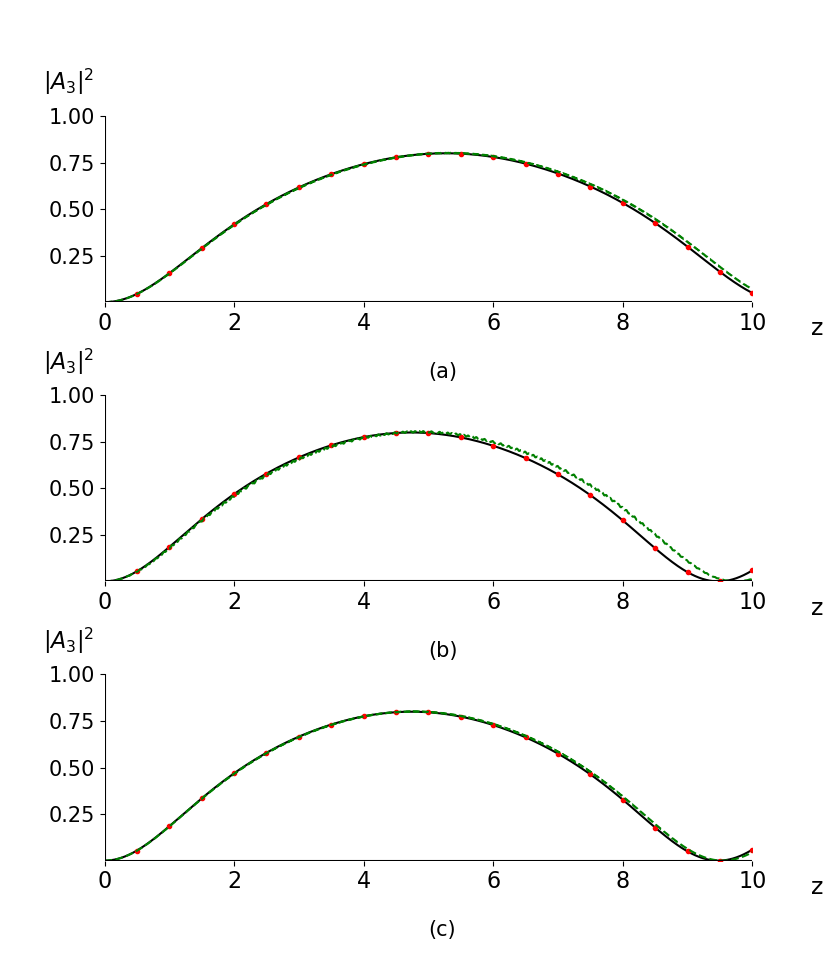
\includegraphics[width=0.5\linewidth]{CascadeI}  
% \caption{The TH intensity evolution computed at $(\gamma;\, \Delta_{21} k)=(6;250)$ (a), $(4;100)$ (b), $(8;400)$ (c) using the numerical solution of the problem \eqref{eq:main2} (solid line), \eqref{eq:ref1} (dashed line) and the analytical solution \eqref{eq:sol} (dotted line).}
% \label{fr:1}
% \end{figure}
}

\textcolor{blue}{
Then there is a very little difference between the problem \eqref{eq:ref1} solution and two other solutions, which arises from the difference of the intensity oscillation period for the solutions of both problems. Therefore, the equation set \eqref{eq:main2} possesses a high approximation of the equation, and the formula \eqref{eq:sol} gives an analytical solution of this problem.
}

\textcolor{blue}{
As it follows from an analytical consideration, the TH intensity maximal value equals \(0.8\), and this value does not depend on the parameters \(\gamma\) and \(\Delta_{21}k\). To verify this, we depict in Fig. \ref{fr:1}b the computer simulation results for the parameters \(\gamma=4\) and \(\Delta_{21}k=100\). We see that the maximal intensity does not change (this statement is also confirmed by Fig.\ref{fr:1}c). Because the phase mismatching is lower than in the previous case (Fig. \ref{fr:1}c), then the difference between two numerical solutions obtained on the base of the original problem and of the modified (simplified) equations increases. In particular, the numerical solution of the problem \eqref{eq:main2} does not describe tiny oscillations, which are observed for the original problem solution (dashed line). Nevertheless, both approaches predict a high energy conversion efficiency for TH.
}

\textcolor{blue}{
To support that the intensity oscillations period depends on the parameter \(\gamma^2/\Delta_{21}k\) we multiply value of \(\gamma\) by \(2\), and \(\Delta_{21}k\) by \(4\) and depict the computer simulation results in Fig. \ref{fr:1}c. We see that the intensity oscillations periods in Figs. \ref{fr:1}b and \ref{fr:1}c are the same. However, with increasing of the phase mismatching, the approximation of the problem solution is better.
}

\textcolor{blue}
{
Thus, the developed analytical solution contains all features of the solution computed on the base of the equation set \eqref{eq:ref1}.
}

\subsection*{Characteristics of the frequency conversion process}
The frequency conversion efficiency is estimated as:
\begin{equation}
\eta_j(z)=\frac{\int\limits_0^{L_t}|A_j(z,t)|^2dt}{\int\limits_0^{L_t}|A_1(z=0,t)|^2dt}.
\end{equation}
Another characteristic, which describes the frequency conversion process is the pulse spectra. They are computed by the formula
\begin{equation}
\hat{A}_j^\omega(z;\omega)=\frac{1}{\sqrt{2\pi}}\int\limits_{0}^{L_t} A_j(z,t)e^{-i\omega t}dt,\,j=1,\,2,\,3
\end{equation}
using the NumPy module \cite{bib:np} of Python Language. We also use the pulse full width at half maximum (FWHM):
\[\tau_j(z)=T_2-T_1,\, |A_j(z,T_l)|^2=0.5|A_j(z,0.5L_t)|^2,\,l=1,\,2,\,T_1<0.5L_t<T_2.\]
 and the corresponding value for spectrum FWHM. Thus, the incident pulse FWHM equals \(1.1772\), and the incident pulse spectrum FWHM equals \(2.357\).

\subsection*{Linear and nonlinear characteristics of crystals}
In Table \ref{tab:2}, we show some characteristics of various crystals at the frequencies corresponding to the frequency conversion processes under consideration. First of all, we write the angle \(\theta\) of the phase matching for the THG due to the cubic nonlinear response of a medium (the second row in Table \ref{tab:2}). The first and second derivatives of wave number with respect to the frequency are presented at the frequencies \(\omega,\, 2\omega\) and \(3\omega\). All data are computed using so-called Sellmeier equations, and they coincide with values, presented in \cite{bib:ri}. We also place the references to the papers, which contain the data, after the names of the crystals. 

\begin{table}
\caption{Characteristics of chosen crystals at \(\lambda=1064\,nm\) of FW}
{\begin{tabular}{|c|c|c|c|c|c|c|} 
\hline
\multicolumn{2}{|c|}{Crystal}& KDP \cite{bib:n26} & ADP \cite{bib:n26} & BBO \cite{bib:c1} & KBBF \cite{bib:c2} &RBBF \cite{bib:c3}\\
\hline
\multicolumn{2}{|c|}{Angle of THG matching $\theta (^{\circ})$} & 64.97 & 66.58 & 37.48 & 31.16 & 33.77 \\
\hline
\multirow{3}{*}{$\frac{d\bar{k}}{d\bar{\omega}}\,(fs/mm)$}& $\bar{\omega}$ & 5084.286 & 5143.42 & 5580.894 & 4951.404 & 4968.198 \\
\cline{2-7}
&$2\bar{\omega}$& 5013.268 & 5063.373 & 5566.836 & 4936.176 & 4955.312 \\
\cline{2-7}
&$3\bar{\omega}$& 5186.888 & 5257.651 & 5889.541 & 5076.076 & 5098.390\\
\hline
\multirow{3}{*}{$\frac{d^2\bar{k}}{d\bar{\omega}^2}\,(fs^2/mm)$}&$\bar{\omega}$ & -12.67 & -16.854 & 42.294 & 14.992 & 17.659 \\
\cline{2-7}
&$2\bar{\omega}$& 67.281 & 74.176 & 120.486 & 57.265 & 58.654 \\
\cline{2-7}
&$3\bar{\omega}$& 124.038 & 139.035 & 229.83 & 96.377 & 98.461 \\
\hline
\end{tabular}
\label{tab:2}}
\end{table}

The second order susceptibility of selected crystals with dependent on the angles \(\theta\) and \(\varphi\), and the incident pulse intensity, at which the coupling coefficient \(\gamma\) is equal to unity at the phase matching angle \(\theta\) (see Table \ref{tab:2}), are shown in Table \ref{tab:3}. The angles are measured between the crystal axis in the uniaxial crystal and wave vector of the FW.

\begin{table}
\caption{The second order susceptibility of some crystals and the incident pulse intensity $I_0$ in dependence of the laser pulse propagation direction with respect to the crystal axis: \((\theta,\,\varphi)\) are spherical coordinates }
{\begin{tabular}{|c|c|c|} 
\hline
Crystal& $\chi^{(2)} (pm/V)$ & $ I_0\,(10^9\,W/cm^2)$ \\
\hline
KDP \cite{bib:c4}& $0.76\sin\theta\sin(2\varphi)$ & 2 \\
\hline
ADP \cite{bib:c4}& $0.76\sin\theta\sin(2\varphi)$ & 2.03 \\
\hline
BBO \cite{bib:c4}& $4.32(\sin\theta-0.07\cos\theta\sin(3\varphi))$ & 0.21 \\
\hline
KBBF \cite{bib:c5}& $0.98\cos\theta\cos(3\varphi)$ & 1.28 \\
\hline
RBBF \cite{bib:c3}& $0.9\cos\theta\cos(3\varphi)$ & 1.63 \\
\hline
\end{tabular}
\label{tab:3}}
\end{table}

\subsection*{Data availability}
The authors declare that all data supporting the findings of this study are available
within this article and its Supplementary Information files.

\subsection*{Code availability}
The custom computer code used to analyse and model the observational data here is available from the corresponding author on request, for the purpose of repeating 
the published results only.

\begin{thebibliography}{0}
\makeatletter
\addtocounter{\@listctr}{33}
\makeatother
\bibitem{bib:np} http://www.numpy.org
\bibitem{bib:n25} Geusic, J. E., Marcos, H. M., Van Uitert, L. Laser oscillations in Nd-doped yttrium aluminum, yttrium gallium and gadolinium garnets. \textit{Applied Physics Letters} \textbf{4}, 182 (1964).
\bibitem{bib:n26} Zernike, F.  Refractive Indices of Ammonium Dihydrogen Phosphate and Potassium Dihydrogen Phosphate between 2000 $\hat{A}$ and $1.5\mu$. \textit{JOSA} \textbf{54}, 1215 (1964).
\bibitem{bib:c1} Tamo\v{s}auskas, G. et al. Transmittance and phase matching of BBO crystal in the \(3 -- 5 \mu m\) range and its application for the characterization of mid-infrared laser pulses. \textit{Optical Materials Express} \textbf{8}, 1410 (2018).
\bibitem{bib:c2} Chen, C. et al. Improved Sellmeier Equations and Phase-Matching Characteristics in Deep-Ultraviolet Region of ${\hbox {KBe}} _ {2}{\hbox {BO}} _ {3}{\hbox {F}} _ {2} $ Crystal. \textit{IEEE Journal of Quantum Electronics} \textbf{44}, 617 (2008).
\bibitem{bib:c3} Chen, C. et al. Deep UV nonlinear optical crystal: $\hbox{RbBe}_2(\hbox{BO}_3)\hbox{F}_2$. \textit{JOSA B} \textbf{26}, 1519 (2009).
\bibitem{bib:c4} Eckardt, R. C., et al. Absolute and relative nonlinear optical coefficients of KDP, KD*P, $\hbox{BaB}_2\hbox{O}_4, \hbox{LiIO}_3, \hbox{MgO: LiNbO}_3$ and KTP measured by phase-matched second-harmonic generation. \textit{IEEE Journal of Quantum Electronics} \textbf{26}, 922 (1990).
\bibitem{bib:c5} Chen, C., et al. The vacuum ultraviolet phase-matching characteristics of nonlinear optical ${\hbox {KBe}} _ {2}{\hbox {BO}} _ {3}{\hbox {F}} _ {2} $. \textit{Applied physics letters} \textbf{68}, 2930 (1996).
\end{thebibliography}


\subsection*{Acknowledgements}
D.M.K. and M.V.F. thank the Russian Science Foundation (Grant 19-11-00113)

\subsection*{Authors Contributions}
V.A.T. has proposed an original idea and method for investigation; D.M.K. and M.V.F. have implemented the theoretical analysis; D.M.K. has made the computer simulations; V.A.T., D.M.K. have taken parts in the results discussing and the paper writing.

\subsection*{Competing interests}
The authors declare no competing interests.

\subsection*{Correspondence and request for materials}
should be addressed to V.A.T. (trofimov@scut.edu.cn)

\end{document} 